\documentclass[]{mathuinsa}

\titleind{
    SISTEM DIAGNOSIS KANKER KULIT BERDASARKAN CITRA DERMOSKOPI MENGGUNAKAN METODE YOLO-V7
    }

\titleeng{
    SKIN CANCER DIAGNOSIS SYSTEM BASED ON DERMOSCOPY IMAGES USING YOLO-V7 METHOD
    }

\fullname{HUDA FEBRIANTO NURROHMAN}
\NIM{H02219010}
\semester{VII}
\examdate{13 Januari 2023}
\degree{Sarjana Matematika}
\yearsubmit{2023}

\firstsupervisor{Dian Candra Rini Novitasari, M. Kom}
\nipfirstsupervisor{198511242014032001}

\firstexaminer{Ahmad Hanif Asyhar, M.Si}
\nipfirstexaminer{19860123201403001}

\secondexaminer{PENGUJI KEDUA}
\nipsecondexaminer{NIP PENGUJI KEDUA}

\thirdexaminer{PENGUJI KETIGA}
\nipthirdexaminer{NIP PENGUJI KETIGA}

\dean{Dr. A. Saepul Hamdani, M.Pd}
\nipdean{197312272005012003}

\tanggalpersetujuan{13 Januari 2023}



\begin{document}
    \cover\titlepage

    % TODO: betulkan hbox yang tumpah-tumpah di sini!
    \approvalpageBeforeExam
    \approvalpage
    \declarepage
    %Setelah Anda selesai Ujian Akhir Skripsi, scan halaman pengesahan yang telah ditandatangani dosen pembimbing, scan juga halaman pernyataan yang telah Anda tandatangani. Selanjutnya simpan hasil scan tersebut dalam bentuk PDF dengan nama pengesahanskripsi.pdf dan pernyataan.pdf (file disimpan di folder yang sama dengan folder dimana file skripsimath.tex tersimpan)
    %Hilangkan karakter % sebelum perintah "\approvalpagescan" dan "\declarepagescan" di bawah ini, dan tambahkan karakter % sebelum perintah "\approvalpage" dan "\declarepage" di atas.
    %\approvalpagescan
    %\declarepagescan


    %-----------------------------------------------------------------
    % motto page \ halaman motto
    %-----------------------------------------------------------------
    \motto
    % \begin{figure}[h] 
    %     \begin{center} 
    %         \includegraphics[scale=0.5]{img/motto.png} 
    %     \end{center}

    % \end{figure}

    \begin{center}
        % Here is the word ``Arabic'' written in Arabic:  \<اَلْعَرَبِيَّةُ>. You can also use the command \verb|\RL{arabic text}| like this: \RL{اَلْعَرَبيَّةُ}.
        $\ldots$ \<وَمَنْ يَتَوَكَّلْ عَلَى اللَّهِ فَهُوَ حَسْبُه> $\ldots$ \\
        {"}Dan barangsiapa yang bertawakkal kepada Allah niscaya Allah akan mencukupkan (keperluan) nya{"}
        (QS. Ath-Thalaq: 3)
    \end{center}


    %-----------------------------------------------------------------
    % preface page \ halaman persembahan
    %-----------------------------------------------------------------
    \acknowledment
    \begin{center}
        \emph\cal{Karya sederhana ini penulis persembahkan \\
        untuk \textit{manusia}}
    \end{center}

    % awal masukan prakata
    \preface
    Segala puji dan syukur penulis panjatkan kepada Allah SWT., yang telah memberikan nikmat karunia dan hidayah-Nya sehingga skripsi dengan judul “SISTEM DIAGNOSIS KANKER KULIT BERDASARKAN CITRA DERMOSKOPI MENGGUNAKAN METODE YOLO-V7”, dapat selesai dengan baik. Berdasarkan hal tersebut, penulis mengucapkan terima kasih yang tak terhingga kepada:

    \begin{enumerate}
        \item Bapak Prof. Akh. Muzakki, M.Ag, Grad.Dip.SEA., M.Phil, Ph.D., selaku rektor Universitas Islam Negeri Sunan Ampel Surabaya.
        \item Bapak Dr. A. Saepul Hamdani, M.Pd., selaku Dekan Fakultas Sains dan Teknologi, Universitas Islam Negeri Sunan Ampel Surabaya.
        \item Ibu Yuniar Farida, M.T., selaku Ketua Program Studi Matematika, Fakultas Sains dan Teknologi, Universitas Islam Negeri Sunan Ampel Surabaya.
        \item Ibu Dian Candra Rini Novitasari, M.Kom., selaku dosen pembimbing skripsi yang senantiasa mengarahkan dan mengingatkan penulis.
        \item Bapak dan Ibu dosen Program Studi Matematika, Fakultas Sains dan Teknologi, Universitas Islam Negeri Sunan Ampel Surabaya.
        \item Seluruh pihak yang terlibat dalam proses pembuatan skripsi ini.
    \end{enumerate}

    Penulis sangat menyadari bahwa karya skripsi ini masih jauh dari kata sempurna. Oleh karena itu, kritik dan saran yang bersifat membangun sangat diharapkan oleh penulis untuk menyempurnakan penulisan skripsi ini. Penulis mengharapkan agar skripsi ini dapat memberikan manfaat pada dunia sains dan masyarakat.
    \vspace{0.8cm}

    \begin{tabular}{p{7cm}c}
        &Surabaya, 13 Januari 2023\\
        &\\
        &\\
        &Penulis
    \end{tabular}


    %-----------------------------------------------------------------
    % table of contents \ daftar isi
    %-----------------------------------------------------------------
    \newpage\phantomsection\addcontentsline{toc}{chapter}{DAFTAR ISI}
    \makeatletter\renewcommand\l@chapter[2]{\ifnum \c@tocdepth >\z@\addpenalty\@secpenalty\addvspace{0em}\setlength\@tempdima{1.4em}\begingroup\parindent \z@ \rightskip \@pnumwidth\parfillskip -\@pnumwidth\leavevmode \bfseries\advance\leftskip\@tempdima\hskip -\leftskip#1\nobreak\ \leaders\hbox{$\m@th\mkern \@dotsep mu\hbox{.}\mkern \@dotsep mu$}\hfil\nobreak\hb@xt@\@pnumwidth{\hss #2}\par\endgroup\fi}\makeatother
    \begin{onehalfspacing}\tableofcontents\end{onehalfspacing}


    %-----------------------------------------------------------------
    % list of tables \ daftar tabel
    %-----------------------------------------------------------------
    % note: jika diperlukan, hapus karakter % sebelum \newpage & \begin
    \newpage\phantomsection\addcontentsline{toc}{chapter}{DAFTAR TABEL}
    \begin{onehalfspacing}\listoftables\end{onehalfspacing}


    %-----------------------------------------------------------------
    % list of figures \ daftar gambar 
    %-----------------------------------------------------------------
    \newpage\phantomsection\addcontentsline{toc}{chapter}{DAFTAR GAMBAR}
    \begin{onehalfspacing}\listoffigures\end{onehalfspacing}


    %-----------------------------------------------------------------
    % indonesian abstract version \ abstrak versi indonesia
    %-----------------------------------------------------------------
    \begin{abstractind}
        Tuliskan abstrak versi indonesia anda di sini!\\
        \noindent
        \textbf{Kata kunci}: Citra dermoskopi, Kanker kulit, Deteksi objek, CNN, YOLO
    \end{abstractind}
    
    
    %-----------------------------------------------------------------
    % english abstract version \ abstrak versi inggris
    %-----------------------------------------------------------------
    \begin{abstracteng}
        Write your indonesian version of abstract here!\\
        \noindent
        \textbf{Kata kunci}: Dermoscopy images, Skin cancer, Object detection, CNN, YOLO
    \end{abstracteng}

    %-----------------------------------------------------------------
    % chapters \ bab-bab
    %-----------------------------------------------------------------
    % note: isi BAB I dapat diedit pada file bab1.tex, dst...
    \chapter{PENDAHULUAN}
    \section{Latar Belakang Masalah}

    Hakikat kehidupan di dunia adalah tidak lepas akan ujian dari Allah SWT. Allah SWT memberikan ujian berupa kesenangan dan kesusahan. Berdasarkan hal tersebut, diperlukan rasa syukur dan sabar. Seseorang yang beruntung akan mendapatkan pahala orang yang bersyukur dalam kondisi senang dan pahala orang bersabar dalam kondisi susah. Sebagaimana firman Allah SWT dalam surah Ibrahim ayat 5, Luqman ayat 31, Saba’ ayat 19, dan Asy-Syu’ara ayat 33 yang berbunyi:

    \begin{flushright}
        \<اِنَّ فِيْ ذٰلِكَ لَاٰيٰتٍ لِّكُلِّ صَبَّارٍ شَكُوْرٍ (٥)>
    \end{flushright}

    Artinya: “Sesungguhnya dalam yang demikian itu terdapat tanda-tanda bagi orang yang bersabar dan bersyukur”. Allah SWT memutuskan ketetapan bagi manusia kecuali hal itu baik baginya \citep{Ramdhan2019}. Seperti kisah Nabi Musa AS. dan kaumnya ketika Allah SWT selamatkan mereka dari Fir’aun dan siksaan yang menghinakan. Berdasarkan hal tersebut, terdapat pelajaran yang besar bagi setiap orang yang bersabar menghadapi kesengsaraan dan bersyukur dalam kenikmatan \citep{Muaziroh2018}. Sebaik-baik hamba ialah orang yang bersabar ketika mendapatkan cobaan dan bersyukur ketika mendapatkan kenikmatan. Sebagaimana kisah Nabi Ayyub AS. ketika beliau menderita penyakit kulit, yaitu kusta atau lepra. Allah SWT menyebutkan kisah Nabi Ayyub AS. dalam surah Al-Anbiya’ ayat 83-84:

    \begin{flushright}
        \begin{RLtext}
            وَاَيُّوْبَ اِذْ نَادٰى رَبَّهٗٓ اَنِّيْ مَسَّنِيَ الضُّرُّ وَاَنْتَ اَرْحَمُ الرّٰحِمِيْنَ ۚ (٣٨) فَاسْتَجَبْنَا لَهٗ فَكَشَفْنَا مَا بِهٖ مِنْ ضُرٍّ وَّاٰتَيْنٰهُ اَهْلَهٗ وَمِثْلَهُمْ مَّعَهُمْ رَحْمَةً مِّنْ عِنْدِنَا وَذِكْرٰى لِلْعٰبِدِيْنَ ۚ (٤٨)
        \end{RLtext}
    \end{flushright}

    Artinya: “Dan (ingatlah kisah) Ayub, ketika ia menyeru Rabbnya: “(Ya Rabbku), sesungguhnya aku telah ditimpa penyakit dan Engkau adalah Rabb Yang Maha Penyayang di antara semua penyayang.” Maka Kamipun memperkenankan seruannya itu, lalu Kami lenyapkan penyakit yang ada padanya dan Kami kembalikan keluarganya kepadanya, dan Kami lipat gandakan bilangan mereka, sebagai suatu rahmat dari sisi Kami dan untuk menjadi peringatan bagi semua yang menyembah Allah”. Nabi Ayyub AS. diuji dengan penyakit kulit sehingga banyak orang menjauhinya. Salah satu penyakit kulit yang umum dan dapat menyebabkan kematian adalah kanker kulit \citep{Nurlitasari2022}. Selain kanker serviks dan kanker payudara, kanker kulit sering ditemukan di Indonesia. Terdapat sekitar 7.8\% kasus kanker kulit per tahun di Indonesia. Kasus kanker kulit yang sering terjadi di Indonesia ialah \textit{Basal Cell Carcinoma} (BCC) sekitar 65.5\%, \textit{Squamous Cell Carcinoma} (SCC) sekitar 23\%, dan \textit{Melanoma} (MEL) sekitar 7.9\%. Meskipun kasus BCC lebih sedikit daripada kasus MEL, akan tetapi jumlah kematian akibat MEL 75\% dari keseluruhan jenis kanker kulit \citep{Fuadah2020a}. MEL merupakan kanker kulit yang paling berbahaya karena dapat menyebabkan kematian. Salah satu penyebab yang menjadikan MEL sangat berbahaya adalah kemampuannya untuk menyebar ke dalam organ lain seperti jantung, hati, dan paru-paru \citep{Nugroho2019}.
    
    Kanker kulit merupakan kondisi pertumbuhan sel yang tidak normal pada kulit. Pertumbuhan sel yang tidak normal akan terus berjalan seiring waktu. Hal ini terjadi karena sering terpapar radiasi sinar \textit{Ultraviolet} (UV) secara langsung. Radiasi sinar UV dapat menembus lapisan luar kulit dan lapisan dalam kulit sehingga dapat merusak sel kulit termasuk sel \textit{Deoxyribonucleic acid} (DNA). DNA yang rusak dapat memicu kesalahan fungsi DNA sehingga DNA bermutasi. Akhirnya, hal ini dapat mengakibatkan pertumbuhan sel yang tidak terkontrol dan disebut kanker kulit \citep{Bhimavarapu2022}. Dampak kanker kulit dapat dikurangi dengan melakukan deteksi pada tahap awal karena morbiditas, mortalitas, dan biaya pengobatan yang sangat berkorelasi dengan tahap penyakit yang diderita. Tahap awal kanker kulit MEL masih merepresentasikan tingkat kematian yang tinggi. Kemudian, tahap lanjut dari MEL akan memperlihatkan gejala yang sangat buruk dan membutuhkan biaya perawatan yang lebih tinggi terutama pengobatan dengan imunoterapi \citep{Janda2022}. Terdapat dua jenis kanker kulit, yaitu \textit{benign} dan \textit{malignant}. \textit{Benign} merupakan kanker kulit yang tidak berbahaya sedangkan \textit{malignant} perlu penanganan khusus bahkan dapat menyebabkan kematian. Sebagian besar \textit{benign} tidak menyebabkan kematian karena \textit{benign} tidak menyebar ke dalam jaringan tubuh lain dan tidak tumbuh di tempat yang sama setelah dihilangkan sehingga \textit{benign} dapat dihilangkan dengan berbagai penanganan medis. Tahi lalat merupakan salah satu contoh dari \textit{benign}. Di sisi lain, \textit{malignant} memiliki tingkat kasus kematian yang cenderung tinggi. \textit{Malignant} mampu bertumbuh secara terus-menerus dan menyebar ke dalam jaringan di sekitarnya. MEL merupakan salah satu contoh dari \textit{malignant}. MEL merupakan jenis paling mematikan dari kanker kulit dan menyumbang 75\% dari kematian akibat kanker kulit. Pada tahap awal, MEL dapat ditangani dengan melakukan pembedahan sehingga pasien memiliki harapan hidup yang tinggi. Akan tetapi, pasien memiliki angka harapan hidup yang rendah jika sudah metastasis \citep{Davis2019}.

    Kanker kulit yang terjadi pada seseorang dapat diidentifikasi melalui gejala yang timbul pada kanker kulit itu sendiri. Gejala kanker kulit biasa disebut sebagai ABCDE oleh para dokter. ABCDE merupakan kependekan dari \textit{Asymmetry}, \textit{Border}, \textit{Color}, \textit{Diameter}, and \textit{Evolve} \citep{Gavrilov2019a}. \textit{Asymmetry} berarti tidak simetris yang menggambarkan terkait bentuk yang muncul pada kanker kulit. \textit{Border} berarti tepi yang merepresentasikan tepian tidak rata, bertekstur kabur, dan kasar pada kanker kulit. \textit{Color} berarti warna yang memperlihatkan kombinasi warna tidak proposional pada kanker kulit. Dengan kata lain, banyak kombinasi yang tidak teratur seperti hitam, coklat, abu-abu, dan merah. Diameter memperhitungkan kisaran diameter pada kanker kulit sekitar 6 mm sampai 0.25 inci. \textit{Evolve} menunjukkan terjadinya perubahan pada sel kanker selama terinfeksi kanker kulit \citep{Saherish2020a}. Dengan fitur ABCDE ini, dokter dapat melihat secara langsung untuk mendeteksi kanker kulit sejak tahap awal. Namun, cara tersebut kurang efisien karena mempertimbangkan penglihatan seseorang yang bisa saja berbeda. Sehingga dikembangkan sistem yang dinamakan \textit{Computer Aided Diagnosys} (CAD) untuk mendeteksi kanker kulit oleh pihak medis. CAD memiliki beberapa tahapan seperti memroses citra digital, ekstraksi fitur, dan klasifikasi \citep{Adyanti2017}.

    Terdapat beberapa penelitian tentang klasifikasi kanker kulit berdasarkan data citra dermoskopi sebelumnya. Ma dan Karki mengimplementasikan \textit{Machine Learning} (ML) untuk mendeteksi \textit{benign} dan \textit{malignant} dengan memanfaatkan fitur ABCD. Ma dan Karki mendapatkan akurasi klasifikasi yang cukup tinggi, yaitu $97.8\%$ menggunakan \textit{Support Vector Machine} (SVM) \citep{Ma2020}. Meskipun ML memiliki akurasi yang cukup tinggi pada beberapa kasus, ML tidak efektif dalam kasus diagnosis yang kompleks dalam praktik klinis. Pada umumnya, metode ML untuk mendeteksi kanker kulit terdiri dari ekstraksi fitur dan klasifikasi terhadap fitur yang sudah diekstraksi. Berdasarkan hal tersebut, ML memiliki keterbatasan pada fitur yang dipakai dan tidak efektif dalam studi kasus yang lebih luas \citep{Wu2022}.

    Alasadi dan Alsafy memanfaatkan pemrosesan citra digital untuk mendeteksi kanker kulit MEL berdasarkan fitur warna, bentuk, dan tekstur sehingga menghasilkan akurasi $98\%$ untuk mengklasifikasikan kanker kulit (\textit{benign} dan \textit{malignant}) dan $93\%$ untuk mengenali tipe MEL. Penelitian Alasadi dan Alsafy menggunakan \textit{Neural Network} (NN) untuk melakukan pengenalan tipe melanoma \citep{Alasadi2015a}. Salah satu perkembangan dari NN adalah \textit{Convolutional Neural Network} (CNN). CNN merupakan bagian dari \textit{deep learning} yang berguna untuk mengolah data citra sehingga CNN dapat mengklasifikasikan citra tanpa melakukan ekstraksi fitur sebelumnya. Karena pada CNN sudah terdapat proses ekstraksi fitur dan pembelajaran fitur. Pada CNN, terdapat berbagai arsitektur, seperti AlexNet, VGG, ResNet, GoogleNet, RCNN, Fast-RCNN, YOLO, dan masih banyak lagi. Nugroho, dkk. melakukan deteksi kanker kulit berdasarkan citra dermoskopi menggunakan CNN sehingga mendapatkan akurasi 78\%. Akurasi yang didapatkan oleh Nugroho, dkk. termasuk baik dengan mempertimbangkan tujuh kelas yang ada pada dataset yang digunakan oleh Nugroho, dkk. dalam penelitiannya \citep{Nugroho2019}. Pada penelitian yang dilakukan Fu’adah, dkk. yang menggunakan CNN, terdapat empat kelas untuk klasifikasi kanker kulit sehingga didapatkan nilai akurasi sebesar 99\% \citep{Fuadah2020a}.

    \textit{You Only Look Once} (YOLO) merupakan salah satu model deteksi objek \textit{real-time} berdasarkan CNN yang dipublikasikan pada tahun 2016 dengan \textit{mean Average Precision} (mAP) sebagai metrik evaluasi. YOLO-v1 mampu mendeteksi objek secara \textit{real-time} namun masih memiliki beberapa batasan, yaitu tidak dapat mendeteksi objek kecil dan akurasi yang kurang baik. YOLO-v1 mendapatkan $63.4$ nilai mAP pada dataset PASCAL VOC 2007 dan $57.9$ nilai mAP pada dataset PASCAL VOC 2012 \citep{Redmon2016a}. YOLO-v2 memperbaiki kelemahan YOLO-v1 dengan menambahkan \textit{batch normalization} untuk meningkatkan mAP dan menggunakan DarkNet-19 untuk memprediksi objek lebih dari satu kelas pada satu sel. DarkNet-19 terdiri dari 19 \textit{convolutional layers} dan 5 \textit{max-pooling layers}. YOLO-v2 juga dapat mendeteksi lebih dari 9000 kelas meskipun berdampak pada mAP. YOLO-v2 mendapatkan $73.4$ nilai mAP pada dataset PASCAL VOC 2012 dan $44$ nilai mAP pada dataset \textit{Microsoft Common Objects in Context} (MS COCO) \citep{Redmon2017}. YOLO-v3 mengganti DarkNet-19 dengan DarkNet-53 disertai \textit{residual blocks} dan \textit{upsampling networks}. Kelebihan YOLO-v3 dapat memprediksi 3 ukuran yang berbeda. YOLO-v3 mendapatka $57.9$ nilai mAP pada dataset MS COCO \citep{Redmon2018}. YOLO-v4 menambahkan \textit{Weighted Residual Connections}, \textit{Cross Mini Batch Normalization}, \textit{Cross Stage Partial Connections}, \textit{Self Adversarial Training}, dan \textit{Mish Activation}. YOLO-v4 mendapatkan $65.7$ nilai mAP pada dataset MS COCO \citep{Bochkovskiy2020}.

    Banyak sekali penelitian sebelumnya yang menggunakan YOLO karena kemampuannya yang dapat mendeteksi objek secara \textit{real-time}. Bahkan, per tahun 2022 sudah terdapat YOLO-v7 meskipun terdapat banyak sekali versi YOLO yang tidak resmi. Kemunculan versi YOLO yang tidak resmi tersebut dikarenakan banyaknya penggemar YOLO yang ingin memodifikasi dan membuat versi YOLO sendiri. Berdasarkan kemunculan banyak versi YOLO sebelumnya, YOLO memiliki berbagai versi yang terus dan masih dikembangkan hingga saat ini. Chhatlani, dkk. melakukan deteksi \textit{melanoma} dan bukan \textit{melanoma} menggunakan YOLOv5 sehingga menghasilkan \textit{Average Precision} (AP) sebesar 89\% untuk kedua kelas, 93\% untuk \textit{melanoma}, dan 83\% untuk bukan \textit{melanoma} \citep{Chhatlani2022a}.
    
    Metode YOLO sudah terbukti dan seringkali menjadi metode yang disarankan untuk melakukan deteksi objek. Perkembangan YOLO dari tahun 2016 hingga tahun 2020 memunculkan banyak variasi dan modifikasi. YOLO sangat bergantung pada pengolahan data saat pembentukan model. Misalnya, ukuran data masukan yang terlalu besar membuat pembentukan model menghabiskan banyak waktu. Di sisi lain, ukuran data masukan yang terlalu kecil membuat YOLO kesulitan untuk mengenali objek pada citra. Sehingga, diperlukan proses \textit{resize} yang tepat untuk menentukan ukuran citra pada proses pembentukan model.
    
    % TODO: Revisi kalimat dengan menyebutkan penelitian siapa saja yang berhasil menggunakan YOLO
    % TODO: Tambahkan keuntungan menggunakan YOLO-v7-Tiny
    Berdasarkan penelitian-penelitian yang sudah ada sebelumnya, algoritma YOLO sangat cepat dan akurat untuk melakukan tugas deteksi objek sehingga penelitian ini menggunakan YOLO-v7 untuk melakukan deteksi kanker kulit berdasarkan citra dermoskopi. Penelitian ini memanfaatkan proses \textit{resize} untuk mengurangi waktu komputasi dan menemukan ukuran citra yang sesuai untuk pembentukan model deteksi kanker kulit. Penelitian ini diharapkan dapat membuat sistem diagnosis kanker kulit menggunakan YOLO-v7 sehingga terdapat alternatif pendeteksian kanker kulit yang efisien.

    \section{Rumusan Masalah}
    Berdasarkan penguraian masalah pada latar belakang penelitian, terdapat rumusan masalah sebagai berikut:
    \begin{enumerate}
        \item Bagaimana proses deteksi kanker kulit menggunakan YOLO-v7 berdasarkan deteksi objek pada data citra dermoskopi?
        \item Bagaimana hasil deteksi kanker kulit menggunakan YOLO-v7 berdasarkan uji coba \textit{batch size}, YOLO-v7, dan YOLO-v7-Tiny?
    \end{enumerate}

    \section{Tujuan Penelitian}
    Berdasarkan kedua rumusan masalah di atas, penelitian ini dilakukan dengan tujuan sebagai berikut:
    \begin{enumerate}
        \item Mengetahui proses deteksi kanker kulit menggunakan YOLO-v7 berdasarkan deteksi objek pada data citra dermoskopi.
        \item Mengetahui hasil deteksi kanker kulit menggunakan YOLO-v7 berdasarkan uji coba \textit{batch size}, YOLO-v7, dan YOLO-v7-Tiny?
    \end{enumerate}

    \section{Manfaat Penelitian}
    Penelitian ini diharapkan dapat memberikan manfaat pada seluruh pihak, seperti yang dipaparkan berikut ini:
    \begin{enumerate}
        \item Manfaat Teoritis
        Penelitian ini diharapkan dapat menjadi referensi untuk para peneliti berikutnya dalam deteksi kanker kulit menggunakan YOLO-v7 berdasarkan deteksi objek pada data citra dermoskopi.

        \item Manfaat Praktis
        \begin{enumerate}
            \item Bagi Penulis
            Meningkatkan pengetahuan penulis dalam menerapkan algoritma YOLO untuk deteksi kanker kulit pada citra dermoskopi.

            \item Bagi Tim Medis
            Meningkatkan efisiensi tim medis untuk mendeteksi kanker kulit dengan kemudahan dan keakuratan yang lebih signifikan.

            \item Bagi Masyarakat
            Meningkatkan waktu diagnosis kanker kulit dan memberikan bahan edukasi kepada masyarakat terkait tingkat bahaya kanker kulit.
        \end{enumerate}
    \end{enumerate}

    \section{Batasan Masalah}
    Mempertimbangkan ruang lingkup permasalahan yang luas, maka penelitian ini menggunakan batasan-batasan masalah sebagai berikut:
    \begin{enumerate}
        \item Metode deep learning yang digunakan pada penelitian ini untuk mendeteksi kanker kulit menggunakan data citra dermoskopi adalah metode YOLO-v7.
        \item Data citra yang digunakan pada penelitian ini untuk mendeteksi kanker kulit adalah data citra dermoskopi.
        \item Kategori kanker yang digunakan pada penelitian ini yaitu \textit{melanoma}, \textit{actinic keratosis}, \textit{nevus}, \textit{basal cell carcinoma}, \textit{squamous cell carcinoma}, \textit{dermatofibroma}, \textit{benign keratosis lesion}, dan \textit{vascular lesion}.
    \end{enumerate}

    \section{Sistematika Penulisan}
    Penelitian ini tersusun atas lima bab yang memuat seluruh isi penelitian dan diringkas pada sistematika penulisan sebagai berikut:
    \begin{enumerate}
        \item BAB I PENDAHULUAN
        memaparkan tentang latar belakang penelitian, rumusan masalah penelitian, tujuan penelitian, manfaat penelitian, dan sistematika penulisan penelitian.
        \item BAB II TINJAUAN PUSTAKA
        memaparkan tentang teori-teori yang digunakan pada penelitian ini berdasarkan jurnal dan buku yang mendukung penelitian ini. Tinjauan pustaka penelitian ini memuat teori tentang kanker kulit dan citra dermoskopi, metode pada tahap pre-processing menggunakan \textit{annotation} dan \textit{resize}, metode pada tahap deteksi kanker kulit menggunakan \textit{You Only Look Once} (YOLO), dan metode pada tahap evaluasi menggunakan \textit{mean Average Precision}.
        \item BAB III METODE PENELITIAN 
        memaparkan tentang proses memperoleh data dan mengolah data sehingga rumusan masalah pada penelitian ini dapat terselesaikan.
        \item BAB IV HASIL DAN PEMBAHASAN
        memaparkan tentang hasil penelitian terkait proses yang terjadi pada deteksi kanker kulit dan analisis hasil yang diperoleh.
        \item BAB V PENUTUP
        memaparkan tentang kesimpulan pada penelitian ini dan saran penulis pada penelitian selanjutnya.
    \end{enumerate}
    \chapter{TINJAUAN PUSTAKA}

\section{Kanker}

    Kanker merupakan pertumbuhan sel yang tidak terkendali pada organ tubuh manusia dan dapat menyebar ke dalam organ tubuh lainnya. Perubahan sel normal menjadi sel kanker disebut sebagai karsinogenesis yang terdiri dari tiga tahap. Tahap pertama merupakan tahap inisiasi yang mengubah ekspresi gen atau bahkan penghapusan bagian DNA akibat mutasi gen. Tahap kedua merupakan tahap promosi yang memulai sel-sel berproliferasi. Tahap terakhir merupakan tahap progresif yang memulai perkembangan sel secara agresif dengan pada jumlah dan ukuran sehingga membentuk tumor primer. Pada tahap ini, sel melakukan invasi dan mulai bermetastasis \citep{Baranwal2021}.

    Ketika sel bertumbuh di luar batas normal dan tidak mengalami kematian, maka akan membentuk tumor \citep{Shedden-Mora2020}. Terdapat dua jenis tumor, yaitu \textit{benign} (tumor jinak) dan \textit{malignant} (tumor ganas). \textit{Benign} tumbuh dengan lambat dan tidak menyebar pada jaringan di sekitarnya. \textit{Benign} tidak berbahaya terhadap tubuh manusia dan prognosisnya baik \citep{Wu2021b}. Sedangkan \textit{malignant} berkembang dan tumbuh serta mengganggu jaringan di sekitarnya. Menghilangkan tumor cenderung sulit meskipun dengan pembedahan. Karena \textit{malignant} tidak berdiferensiasi dengan baik dan tidak matang sehingga menyebar ke dalam jaringan di sekitarnya \citep{li2022epidemiology}. Akibatnya, sering terjadi pertumbuhan tumor lagi setelah pembedahan. Metastasis sering terjadi karena menyebar ke dalam jaringan di sekitarnya. Jika tidak dilakukan pembedahan, terapi radiasi, atau terapi kemo maka akan mengakibatkan kematian. Terkait \textit{malignant}, prognosis bergantung pada waktu diagnosis, derajat kemajuan, dan metastasis \citep{Park2022}.

    Terdapat beberapa penanganan medis untuk mengatasi sel kanker yang berkembang, yaitu pembedahan, terapi kemo, terapi hormon, terapi biologis, dan terapi radiasi. Pembedahan dilakukan oleh tenaga medis dengan memotong sel kanker. Terapi kemo merupakan penanganan sel kanker dengan pemberian obat untuk membunuh sel kanker \citep{Strobel2019}. Terapi hormon digunakan untuk menghentikan hormon yang dibutuhkan oleh sel kanker dalam berkembang. Terapi biologis bekerja dengan sistem kekebalan tubuh untuk menangani sel kanker atau menangani efek samping dari sel kanker \citep{Waks2019}. Terapi radiasi menggunakan sinar-X untuk membunuh sel kanker \citep{Wu2021}. Akan tetapi, berbagai metode tersebut belum tentu sesuai untuk setiap orang dan terdapat efek samping dalam melakukan setiap metode tersebut.

\section{Kanker Kulit}
Kanker kulit merupakan penyakit yang mengubah sel normal pada kulit menjadi sel kanker. Sel kanker akan tumbuh pada kulit secara terus menerus dan biasanya tidak simetris. Kanker kulit memiliki struktur yang tidak umum dengan diferensiasi sel pada tingkat kromatin, nukleus, dan sitoplasma. Hal ini karena terdapat kerusakan pada DNA. Kerusakan pada DNA dapat terjadi karena paparan sinar UV secara berlebihan. Radiasi sina UV dapat menembus bagian dalam kulit sehingga dapat membunuh sel-sel kulit termasuk DNA pada sel. Kerusakan pada DNA dapat menyebabkan malfungsi sehingga DNA pada sel bermutasi \citep{Nugroho2019}.

    \subsection{\textit{Melanoma} (MEL)}
    \textit{Melanoma} termasuk dalam kanker kulit yang sangat berbahaya. Kanker kulit \textit{melanoma} dapat menyebar ke dalam organ tubuh lain. \textit{Melanoma} berasal dari melanosit. Melanosit merupakan sel penghasil melanin yang ada pada kulit. \textit{Melanoma} memiliki bentuk yang tidak normal, tidak simetris, dan memiliki lebih dari satu warna. Tahi lalat yang terkena \textit{melanoma} dapat menimbulkan rasa gatal dan mengeluarkan darah. \textit{Melanoma} biasanya ditemukan di vulva, mata, kulit, sinus, paru-paru, tenggorokan, saluran pencernaan, dan saluran reproduksi. Selain itu, kanker kulit \textit{melanoma} juga dapat ditemukan di bagian anus dan rektum. \textit{Melanoma} lebih sering ditemukan di tubuh seorang pria daripada seorang wanita. Hampir sama dengan jenis kanker kulit lain, penyebab utama kemunculan kanker kulit \textit{melanoma} karena mutasi genetik akibat radiasi sinar UV. Sinar UV tidak merusak DNA secara langsung, akan tetapi membentuk spesies oksigen reaktif sepanjang fotoreseptor non-DNA pada tubuh. Radikal oksigen yang dihasilkan menyebabkan kerusakan dan fragmentasi DNA sehingga mengakibatkan mutasi gen \citep{Sang2019}. Kanker kulit \textit{melanoma} seperti terlihat pada Gambar \ref{fig:mel}.
    \begin{figure}[H] 
        \begin{center} 
            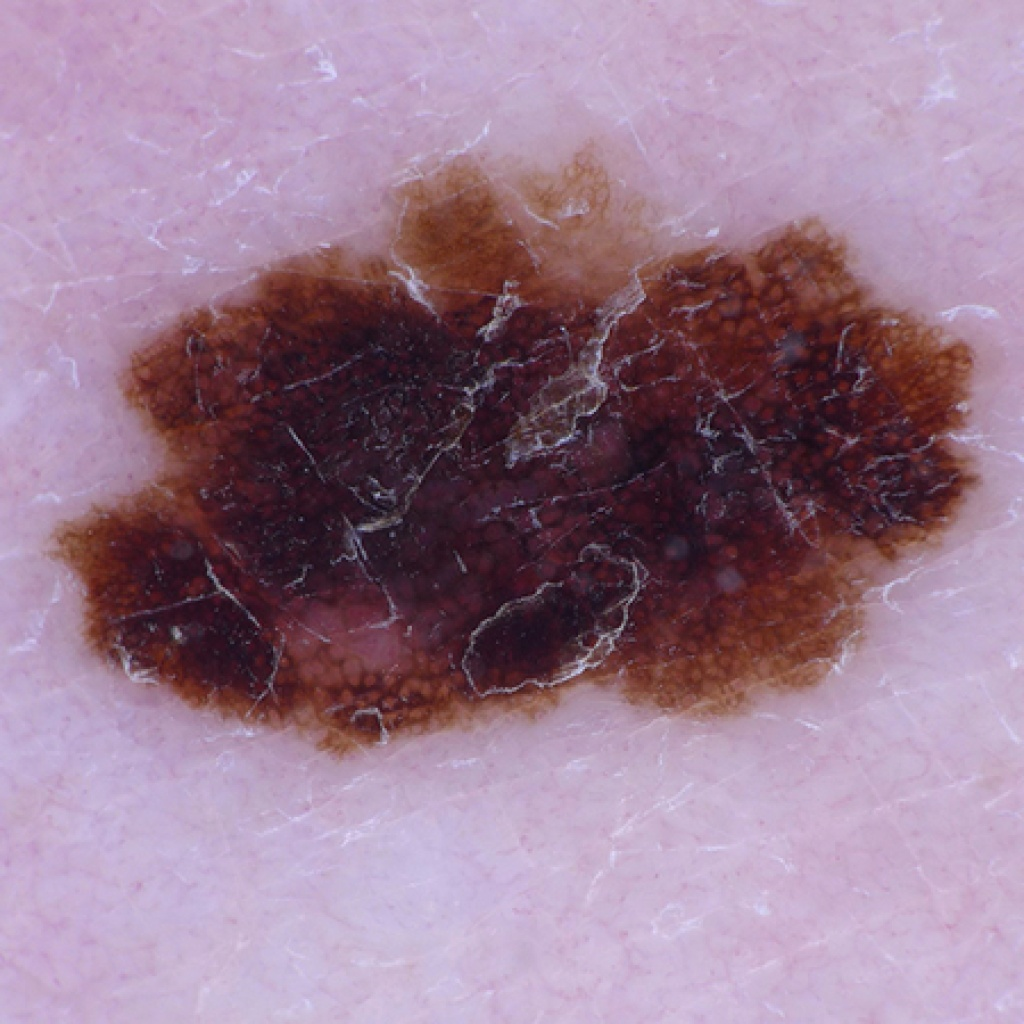
\includegraphics[width=4cm]{../img/Skin Cancer MEL - Latex.jpg}
            \caption{Kanker kulit \textit{melanoma}} 
            \label{fig:mel}
            Sumber: \citep{Codella2018,Combalia2019,Tschandl2018}
        \end{center} 
    \end{figure}

    \subsection{\textit{Actinic Keratosis} (AK)}
    AK merupakan kanker kulit yang sangat umum diderita. Paparan sinar UV yang sangat tinggi pada tubuh dapat menyebabkan kemunculan AK, seperti pada bagian wajah, kulit kepala, leher, punggung tangan, dan lengan. AK memiliki kemungkinan berevolusi menjadi SCC, akan tetapi tidak memungkinkan untuk memprediksi setiap lesi. Oleh karena itu, pengobatan AK sangat penting untuk menghindari perubahannya menjadi SCC. Seseorang yang berusia lebih dari 40 tahun memiliki kecenderungan untuk terkena AK daripada seseorang yang lebih muda \citep{Dianzani2020}. Kanker kulit actinic keratosis seperti terlihat pada Gambar \ref{fig:ak}.
    \begin{figure}[H] 
        \begin{center} 
            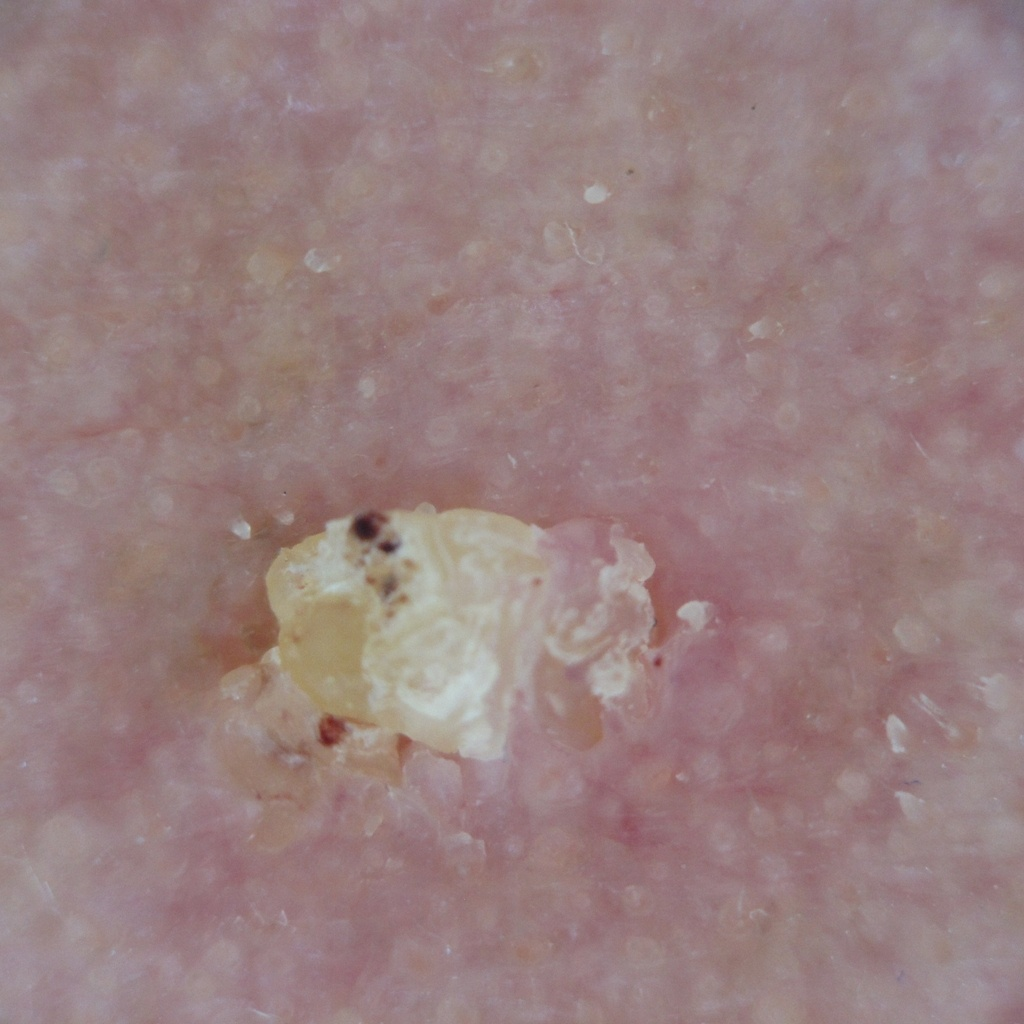
\includegraphics[width=4cm]{../img/Skin Cancer AK - Latex.jpg}
            \caption{Kanker kulit \textit{actinic keratosis}} 
            \label{fig:ak}
            Sumber: \citep{Codella2018,Combalia2019,Tschandl2018}
        \end{center} 
    \end{figure}

    \subsection{\textit{Melanocytic Nevus} (NV)}
    NV merupakan benign yang berasal dari melanosit, sel dendritik yang menghasilkan pigmen, dan biasanya ditemukan di antara keratinosit yang berada pada lapisan basal epidermis. NV yang bertumbuh sangat berbahaya karena berpotensi menjadi melanoma. NV memiliki ciri-ciri seperti tahi lalat. Jika NV sering terpapar polusi, sinar UV, dan bahan kimia berbahaya dapat berpotensi menjadi melanoma. Kanker kulit jenis ini memberikan efek bagi seseorang yang terkena komplikasi, seperti gangguan saraf, kejang, pingsan, dan muntah \citep{Fuadah2020a}. Kanker kulit nevus seperti terlihat pada Gambar \ref{fig:nv}.
    \begin{figure}[H] 
        \begin{center} 
            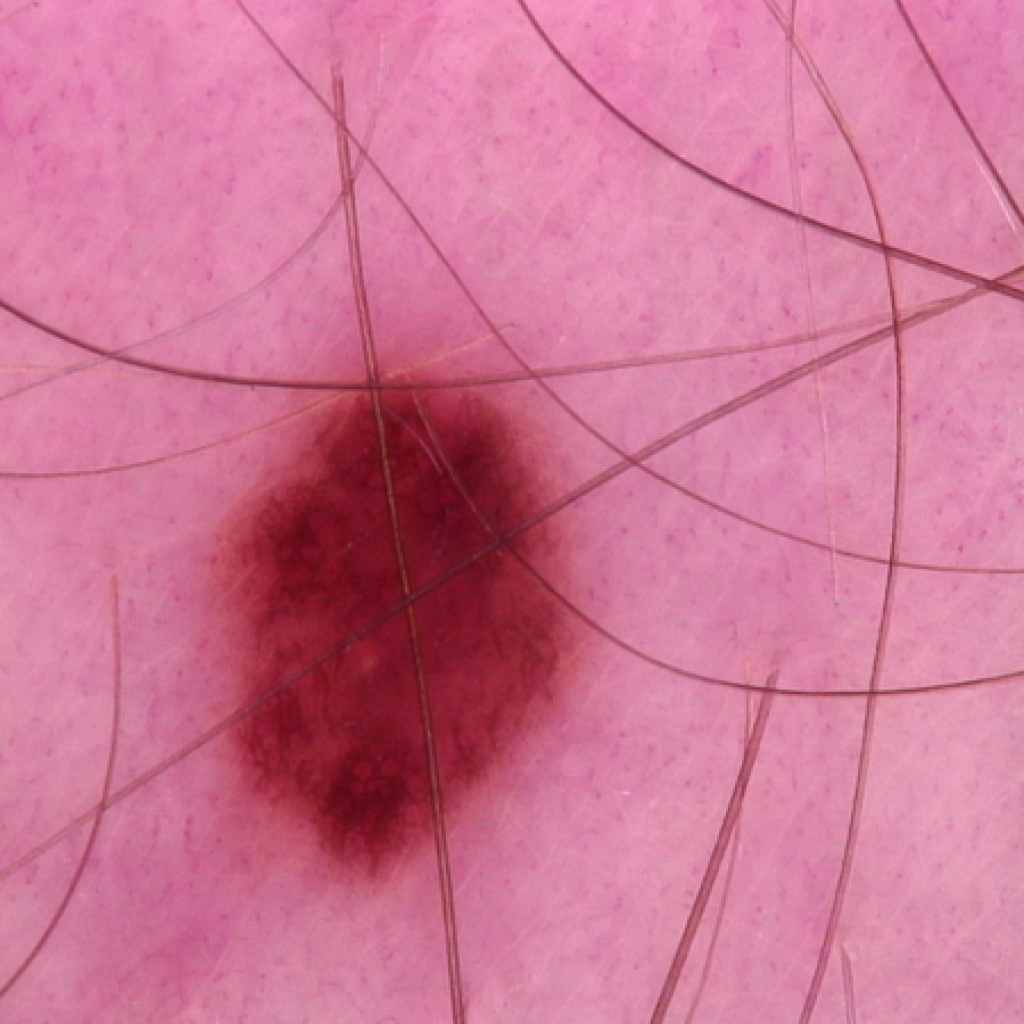
\includegraphics[width=4cm]{../img/Skin Cancer NV - Latex.jpg}
            \caption{Kanker kulit \textit{melanocytic nevus}} 
            \label{fig:nv}
            Sumber: \citep{Codella2018,Combalia2019,Tschandl2018}
        \end{center} 
    \end{figure}

    \subsection{\textit{Basal Cell Carcinoma} (BCC)}
    BCC merupakan kanker kulit yang dari sel-sel basal di dekat persimpangan epidermis-dermis. Kanker kulit jenis ini tumbuh dengan lambat dan tidak bermigrasi. Kemunculan BCC seringkali karena paparan sinar matahari secara langsung dan berlebihan dan biasanya terdapat pada bagian wajah atau leher. Pria dan orang yang semakin tua memiliki presentase lebih tinggi untuk terkena BCC. Diet energi tinggi (khususnya lemak tinggi, vitamin rendah), bahan kimia berbahaya, dan paparan debu juga dapat menyebabkan munculnya BCC. Dalam praktiknya, BCC dibagi menjadi empat jenis, yaitu jenis dangkal, nodular, pigmen, dan titik keras \citep{Sang2019}. Kanker kulit BCC seperti terlihat pada Gambar \ref{fig:bcc}.
    \begin{figure}[H] 
        \begin{center} 
            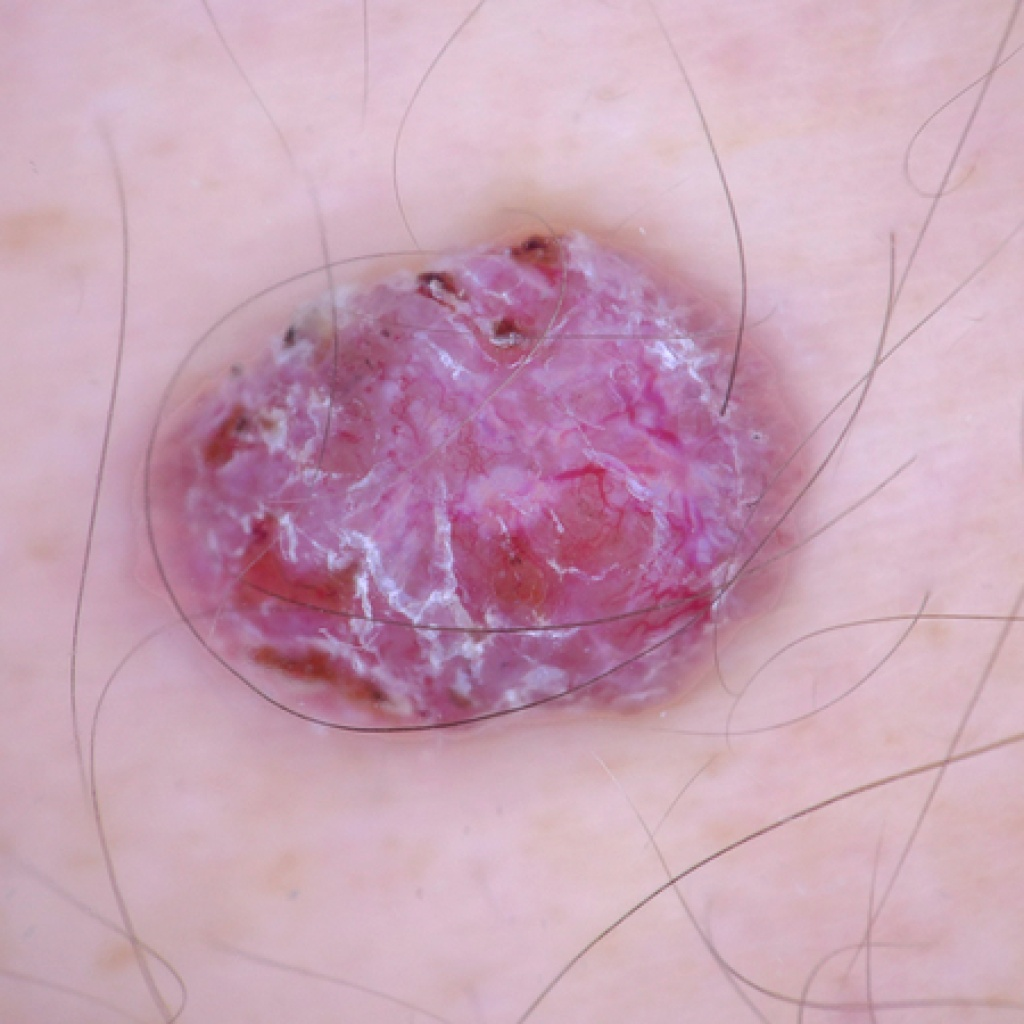
\includegraphics[width=4cm]{../img/Skin Cancer BCC - Latex.jpg}
            \caption{Kanker kulit \textit{basal cell carcinoma}} 
            \label{fig:bcc}
            Sumber: \citep{Codella2018,Combalia2019,Tschandl2018}
        \end{center} 
    \end{figure}

    \subsection{\textit{Squamous Cell Carcinoma} (SCC)}
    SCC merupakan tipe kanker kulit yang tidak agresif. Kanker kulit jenis ini tumbuh dengan lambat. Terapi tanpa pembedahan dapat menangani SCC jika didiagnosis lebih awal. Karena benign dapat bertumbuh dengan terus menerus serta menyebar ke tulang, jaringan, dan bahkan kelenjar getah bening jika tidak ditangani sejak awal \citep{Fuadah2020a}. SCC kebanyakan diderita oleh seseorang yang berusia lebih dari 60 tahun dan berjenis kelamin pria. Daerah invasi SCC dapat dibagi menjadi tiga bagian, yaitu dangkal, dalam, dan tipe transfer \citep{Sang2019}. Kanker kulit SCC seperti terlihat pada Gambar \ref{fig:scc}.
    \begin{figure}[H] 
        \begin{center} 
            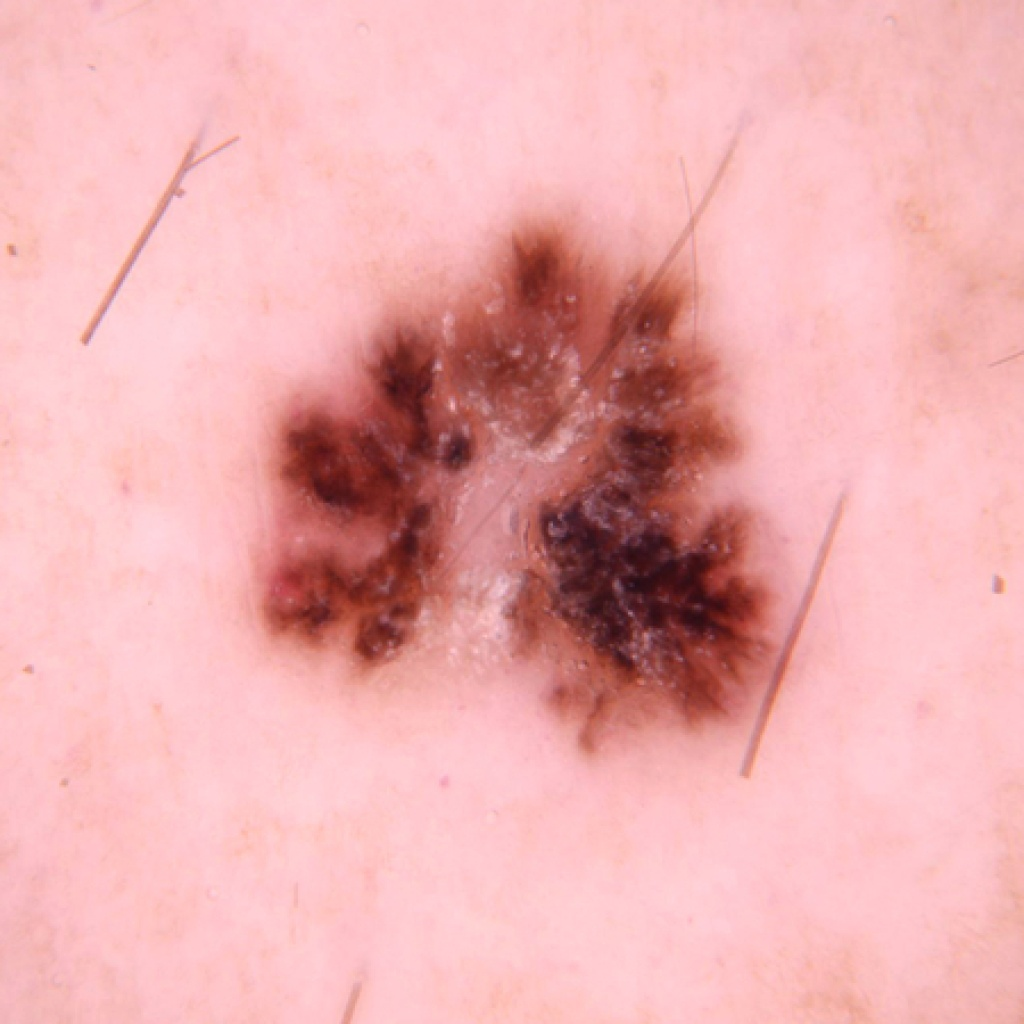
\includegraphics[width=4cm]{../img/Skin Cancer SCC - Latex.jpg}
            \caption{Kanker kulit \textit{squamous cell carcinoma}} 
            \label{fig:scc}
            Sumber: \citep{Codella2018,Combalia2019,Tschandl2018}
        \end{center} 
    \end{figure}

    \subsection{\textit{Dermatofibroma} (DF)}
    DF termasuk ke dalam kategori benign. Kanker kulit jenis ini muncul karena pertumbuhan campuran dari jenis sel di lapisan dermis kulit secara berlebih. Gejala defmatofibroma muncul setelah mengalami beberapa trauma kulit ringan, seperti luka tusuk. Dermatofibroma berukuran sekitar 2-3 mm, berwarna coklat keunguan, berstruktur keras, dan menimbulkan rasa nyeri ketika ditekan \citep{Fuadah2020a}. Kanker kulit DF seperti terlihat pada Gambar \ref{fig:df}.
    \begin{figure}[H] 
        \begin{center} 
            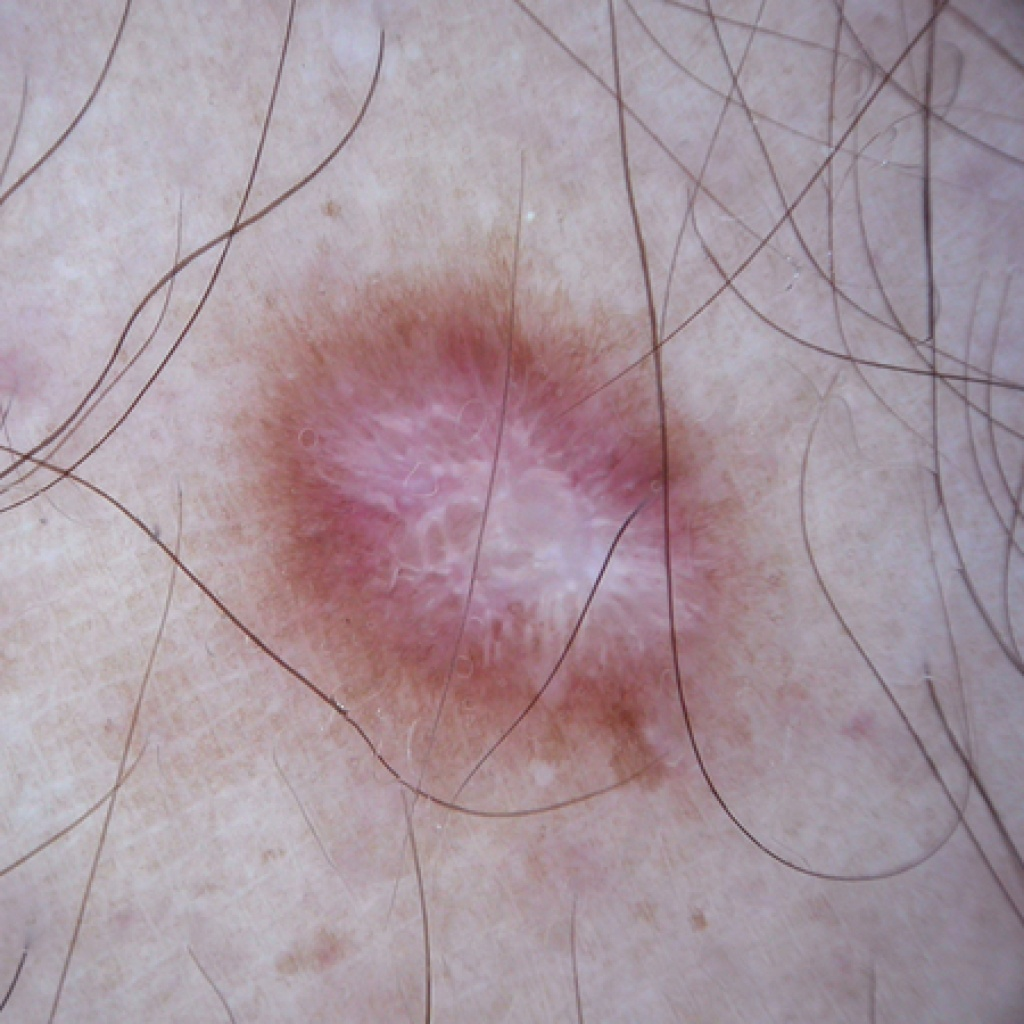
\includegraphics[width=4cm]{../img/Skin Cancer DF - Latex.jpg}
            \caption{Kanker kulit \textit{dermatofibroma}} 
            \label{fig:df}
            Sumber: \citep{Codella2018,Combalia2019,Tschandl2018}
        \end{center} 
    \end{figure}

    \subsection{\textit{Benign Keratosis Lesion} (BKL)}
    BKL merupakan kanker kulit yang tidak berbahaya dan tumbuh dengan warna coklat, hitam, atau coklat lilin. BKL cenderung tidak berbahaya dan tidak memerlukan perawatan khusus. Tampilan umum dari BKL berupa bercak bulat atau oval yang seakan-akan menempel pada kulit. Kanker kulit jenis ini lebih sering terjadi seiring bertambahnya usia. Daerah kulit yang mengandung rambut dan mukosa sering kali menjadi tempat tumbuhnya BKL. Kanker kulit jenis ini juga ditemukan di daerah genital pria \citep{Hall2019}. Kanker kulit BKL seperti terlihat pada Gambar \ref{fig:bkl}.
    \begin{figure}[H] 
        \begin{center} 
            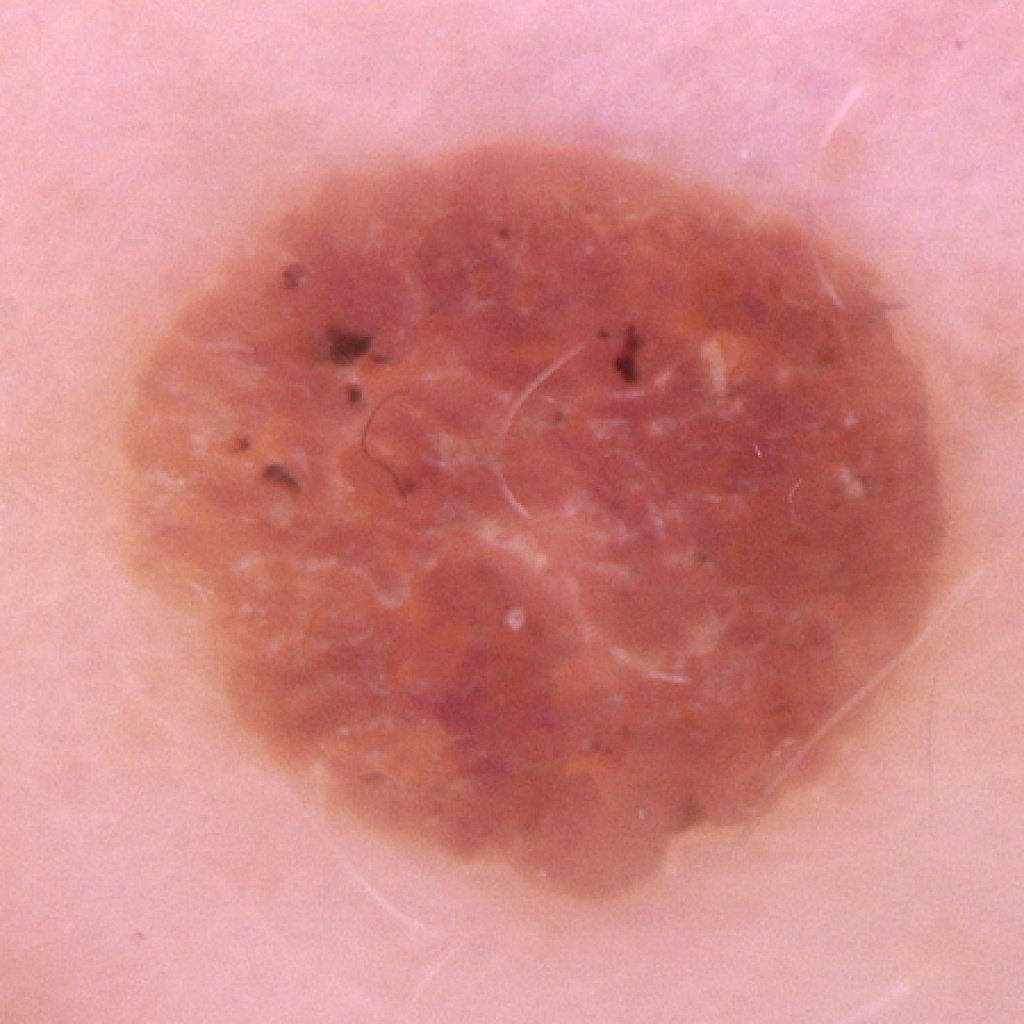
\includegraphics[width=4cm]{../img/Skin Cancer BKL - Latex.jpg}
            \caption{Kanker kulit \textit{benign keratosis lesion}} 
            \label{fig:bkl}
            Sumber: \citep{Codella2018,Combalia2019,Tschandl2018}
        \end{center} 
    \end{figure}

    \subsection{\textit{Vascular Lesion} (VASC)}
    VASC atau yang lebih dikenal sebagai tanda lahir merupakan kanker kulit yang ada pada kulit dan jaringan di bawahnya \citep{Balas2018}. Kanker kulit jenis ini relatif umum terjadi. Terdapat tiga kategori utama dari VASC, yaitu Hemangioma, Malformasi Vaskular, dan Granuloma Piogenik. Ketiga jenis tanda lahir ini terlihat serupa, meskipun ketiganya memiliki perawatan yang berbeda-beda. Hemangioma merupakan jenis kanker kulit yang umum pada anak-anak. Seringkali Hemangioma dapat dipantau oleh dokter kulit atau dokter anak karena kanker kulit jenis ini tumbuh secara alami dan tanpa perawatan. Meskipun tidak banyak Hemangioma yang perlu perawatan khusus karena berada pada daerah yang tidak tepat. Malformasi vaskular merupakan kesalahan kongenital dalam pembentukan pembuluh darah. Malformasi vaskular memerlukan perawatan khusus karena terkait dengan kesalahan fungsi pada pembuluh darah. Granuloma piogenik merupakan kanker kulit tidak berbahaya yang terbentuk sebagai respon terhadap cedera jaringan lokal. Kanker kulit jenis ini umumnya muncul pada anak-anak dan ibu hamil pada daerah mulut dan ujung jari \citep{Rastogi2020}. Kanker kulit VASC seperti terlihat pada Gambar \ref{fig:vasc}.
    \begin{figure}[H] 
        \begin{center} 
            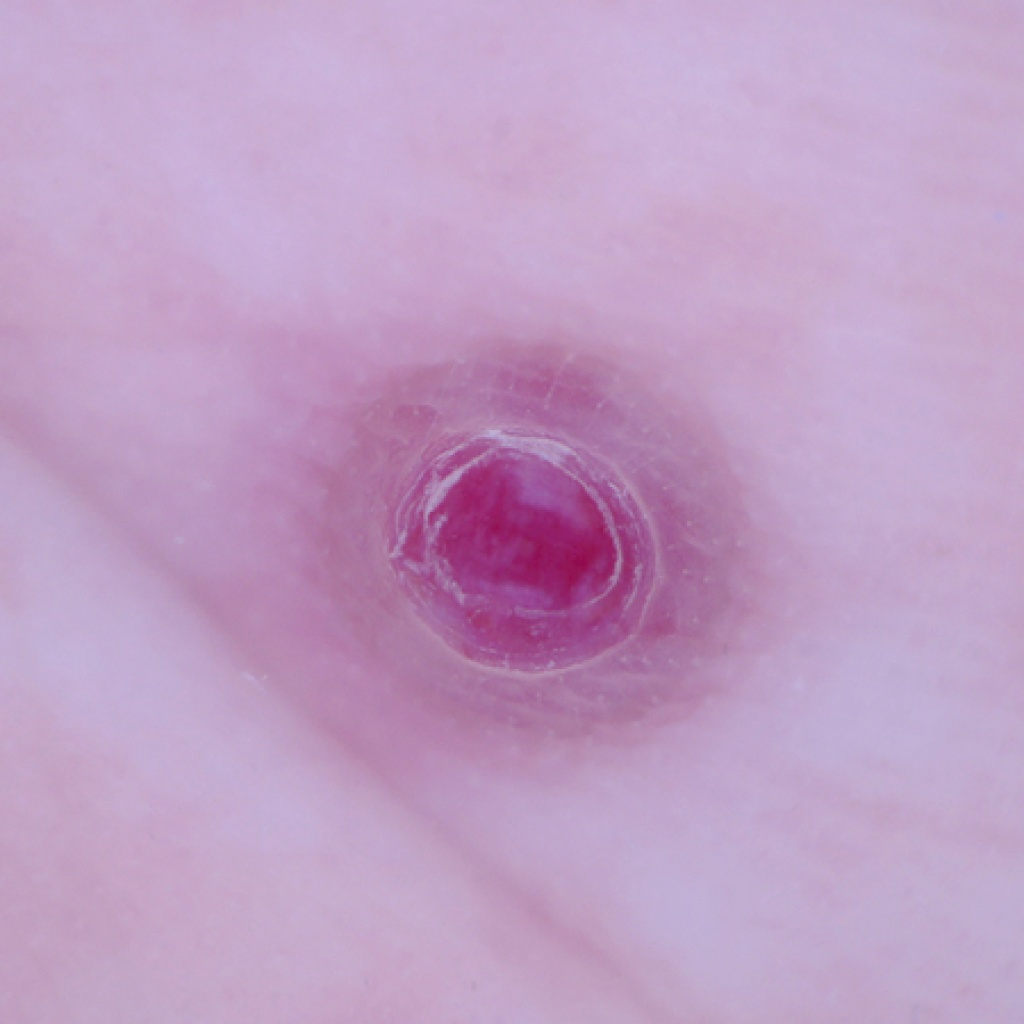
\includegraphics[width=4cm]{../img/Skin Cancer VASC - Latex.jpg}
            \caption{Kanker kulit \textit{vascular lesion}} 
            \label{fig:vasc}
            Sumber: \citep{Codella2018,Combalia2019,Tschandl2018}
        \end{center} 
    \end{figure}

\section{Citra Digital}
Sebagian besar informasi didapatkan dalam bentuk gelombak elektrik dan sinyal. Informasi dapat diubah ke dalam bentuk sinyal dua dimensi atau biasa disebut sebagai citra. Citra digital merupakan representasi dari fungsi intensitas cahaya dalam bentuk distkit pada ruang dua dimensi. Pada citra digital terdapat beberapa elemen baris dan kolom yang disebut piksel. Piksel pada citra memiliki atribut koordinat $(x,y)$ dan amplitudo $(x,y)$. Koordinat $(x,y)$ merepresentasikan letak piksel dalam sebuah citra digital. Sedangkan amplitudo $(x,y)$ menunjukkan intensitas warna yang ada pada citra \citep{Ratna2020}. Sebuah citra digital dapat dilihat sebagai gambaran visual dari matriks yang berisi bilangan bulat (integer). Bilangan bulat tersebut menunjukkan derajat keabuan untuk citra tingkat abu-abu dan menunjukkan warna untuk citra tingkat warna \citep{Blackledge2005,Septiaji2018}.

Citra dapat direpresentasikan sebagai fungsi dari dua variabel $f(x,y)$ berdasarkan tingkat keabuan $(x,y)$. Sehingga citra tersebut dapat diubah menjadi fungsi diskrit sebagai citra digital seperti terlihat pada Persamaan (\ref{eq:citra}).

\begin{align}
    f_{ij} \textnormal{ dimana } f_{ij} &\equiv f(x_i, y_i)
    \label{eq:citra}
\end{align}

$f_{ij}$ merupakan nilai fungsi pada $x=x_i$ dan $y=y_i$ sehingga bisa didefinisikan sebagai matriks atau array dua dimensi seperti pada Persamaan \ref{eq:citra2}.

\begin{align}
    f_{ij} &=
    \begin{bmatrix}
        f_{11} &f_{12} &\cdots &f_{1n}\\
        f_{21} &f_{12} &\cdots &f_{1n}\\
        \vdots &\vdots &\ddots &\vdots\\
        f_{n1} &f_{n2} &\cdots &f_{nn}\\
    \end{bmatrix}
    \label{eq:citra2}
\end{align}

    \subsection{Citra Warna}
    Citra RGB merupakan citra digital yang memiliki tiga kanal warna, yaitu Red, Green, Blue (RGB). Setiap lapisan warna, masing-masing memiliki nilai piksel antara 0 sampai 255. Pada umumnya, nilai piksel ini tersimpan pada memori komputer atau berkas tertentu dalam bentuk 8-bit atau $2^8$ warna. Gambar \ref{fig:color} merupakan contoh citra RGB \citep{Septiaji2018}.

    \begin{figure}[H]
        \begin{center}
            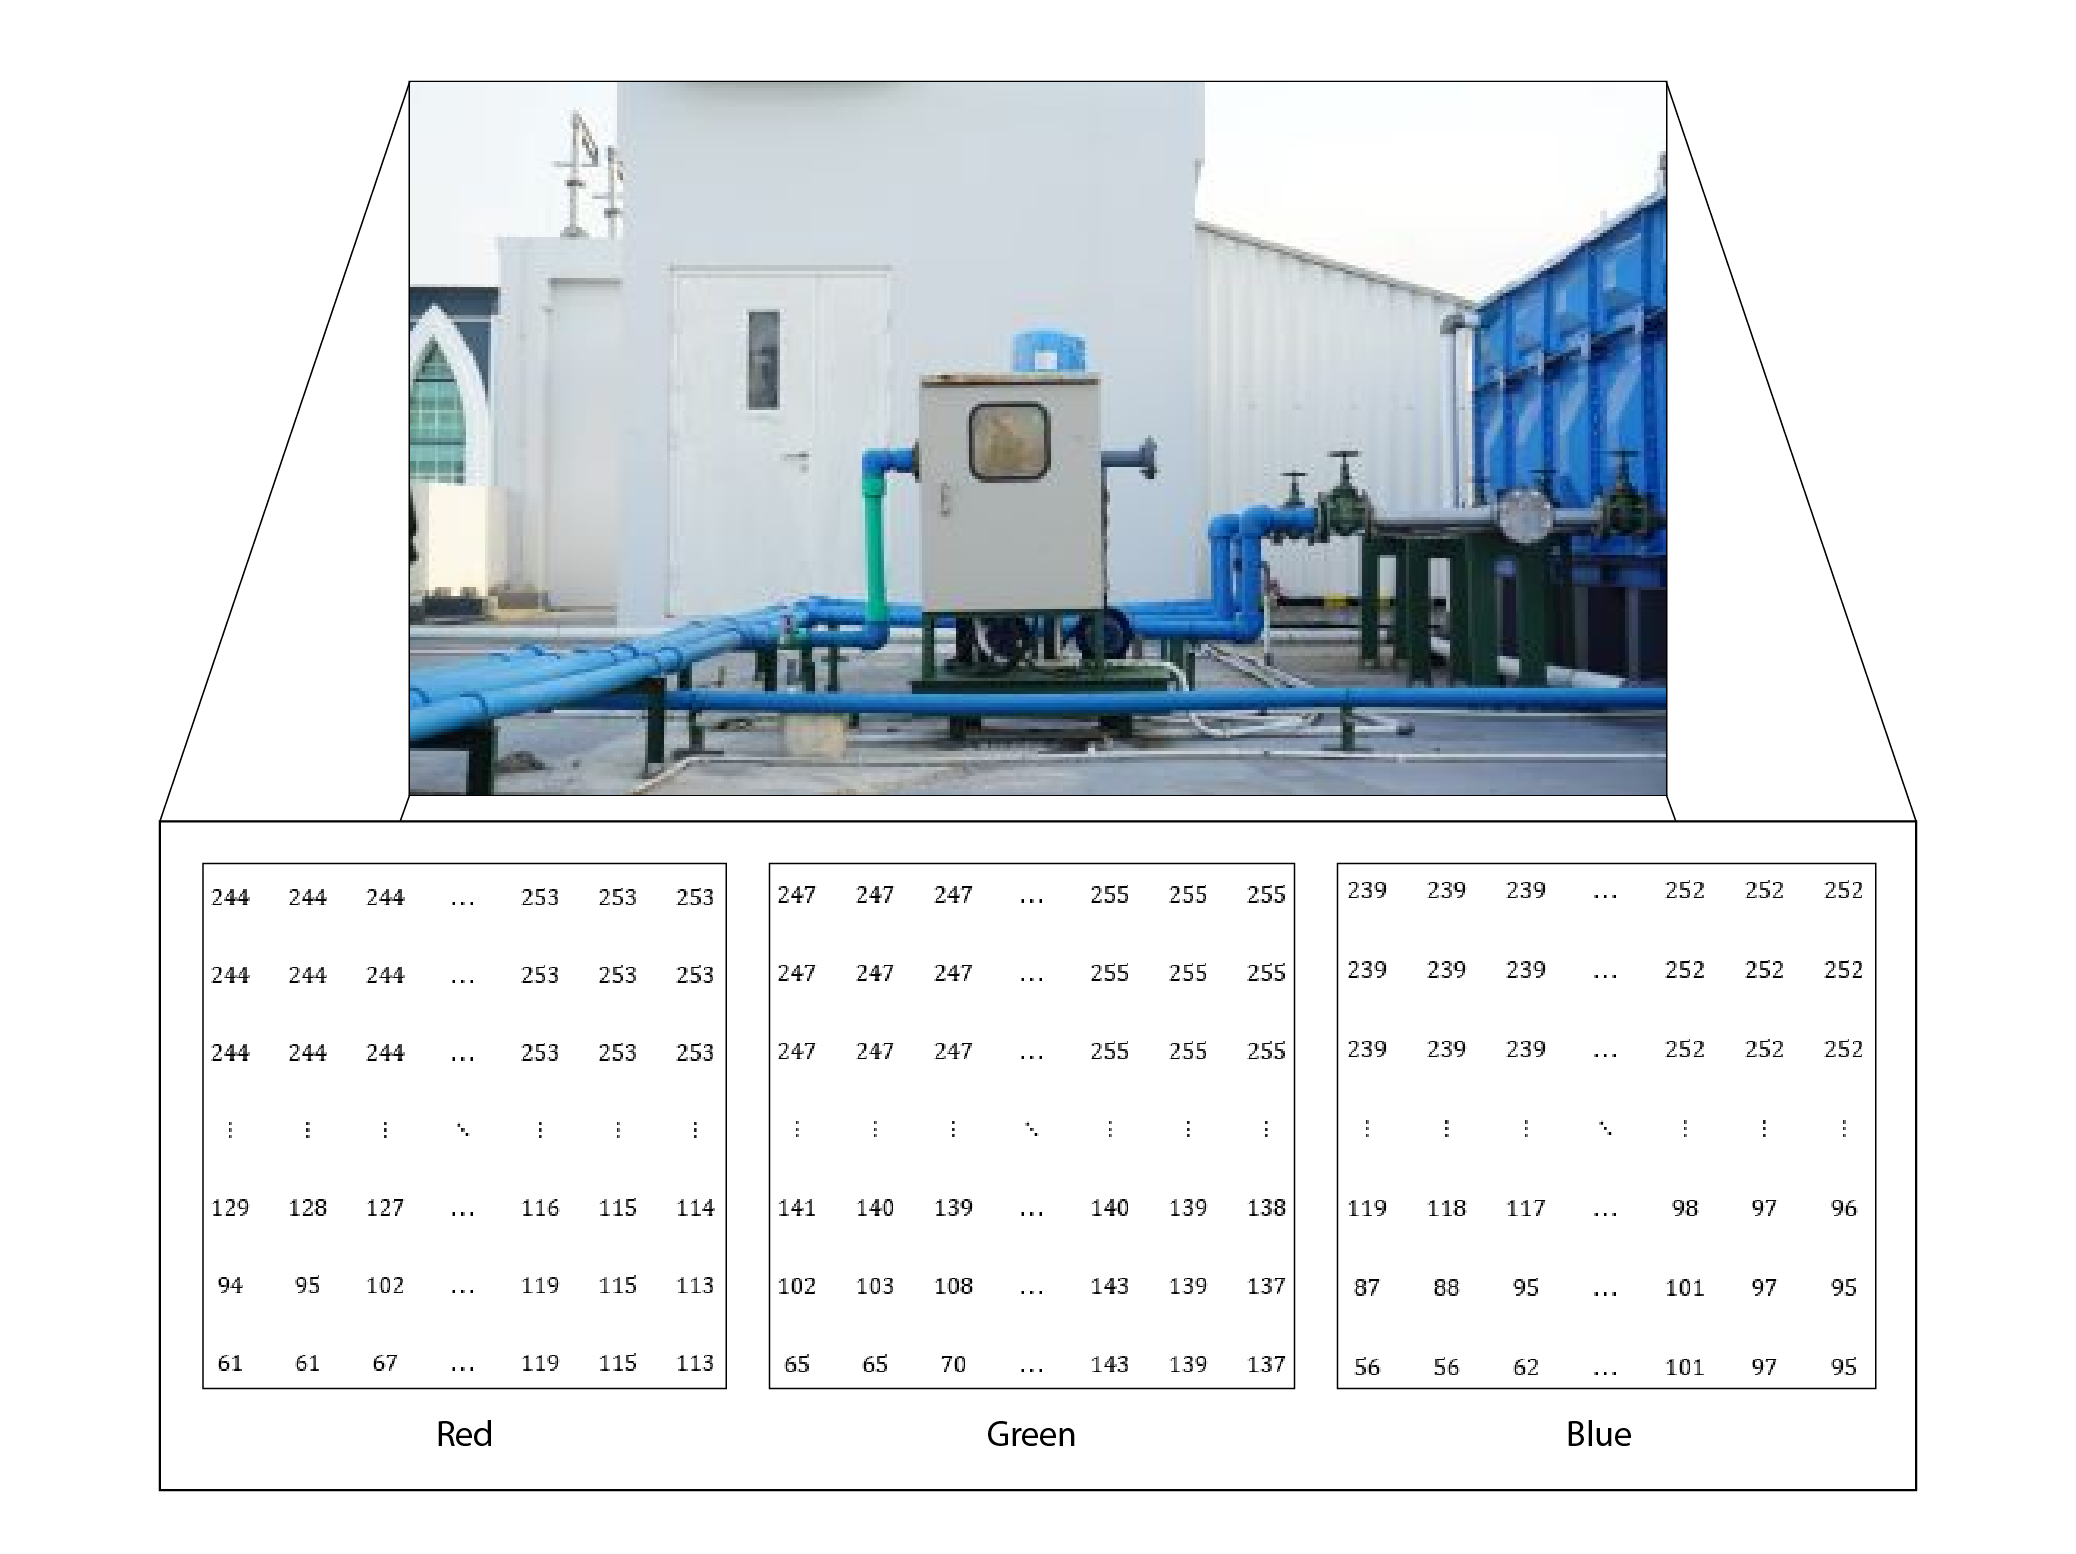
\includegraphics[width=8cm]{../img/Color - Latex.png}
            \caption{Citra warna beserta nilai pikselnya}
            \label{fig:color}
            Sumber: \citep{Kusumanto2011}
        \end{center}
    \end{figure}

    \subsection{Citra Skala Abu-Abu}
    Citra skala abu-abu merupakan citra yang memiliki satu kanal warna, yaitu menunjukkan intensitas derajat keabuan itu sendiri. Pada umumnya, nilai piksel yang dimiliki citra skala abu-abu berkisar antara 0 sampai 255 \citep{Kusumanto2011}. Gambar \ref{fig:grayscale} merupakan salah satu contoh citra skala abu-abu.

    \begin{figure}[H]
        \begin{center}
            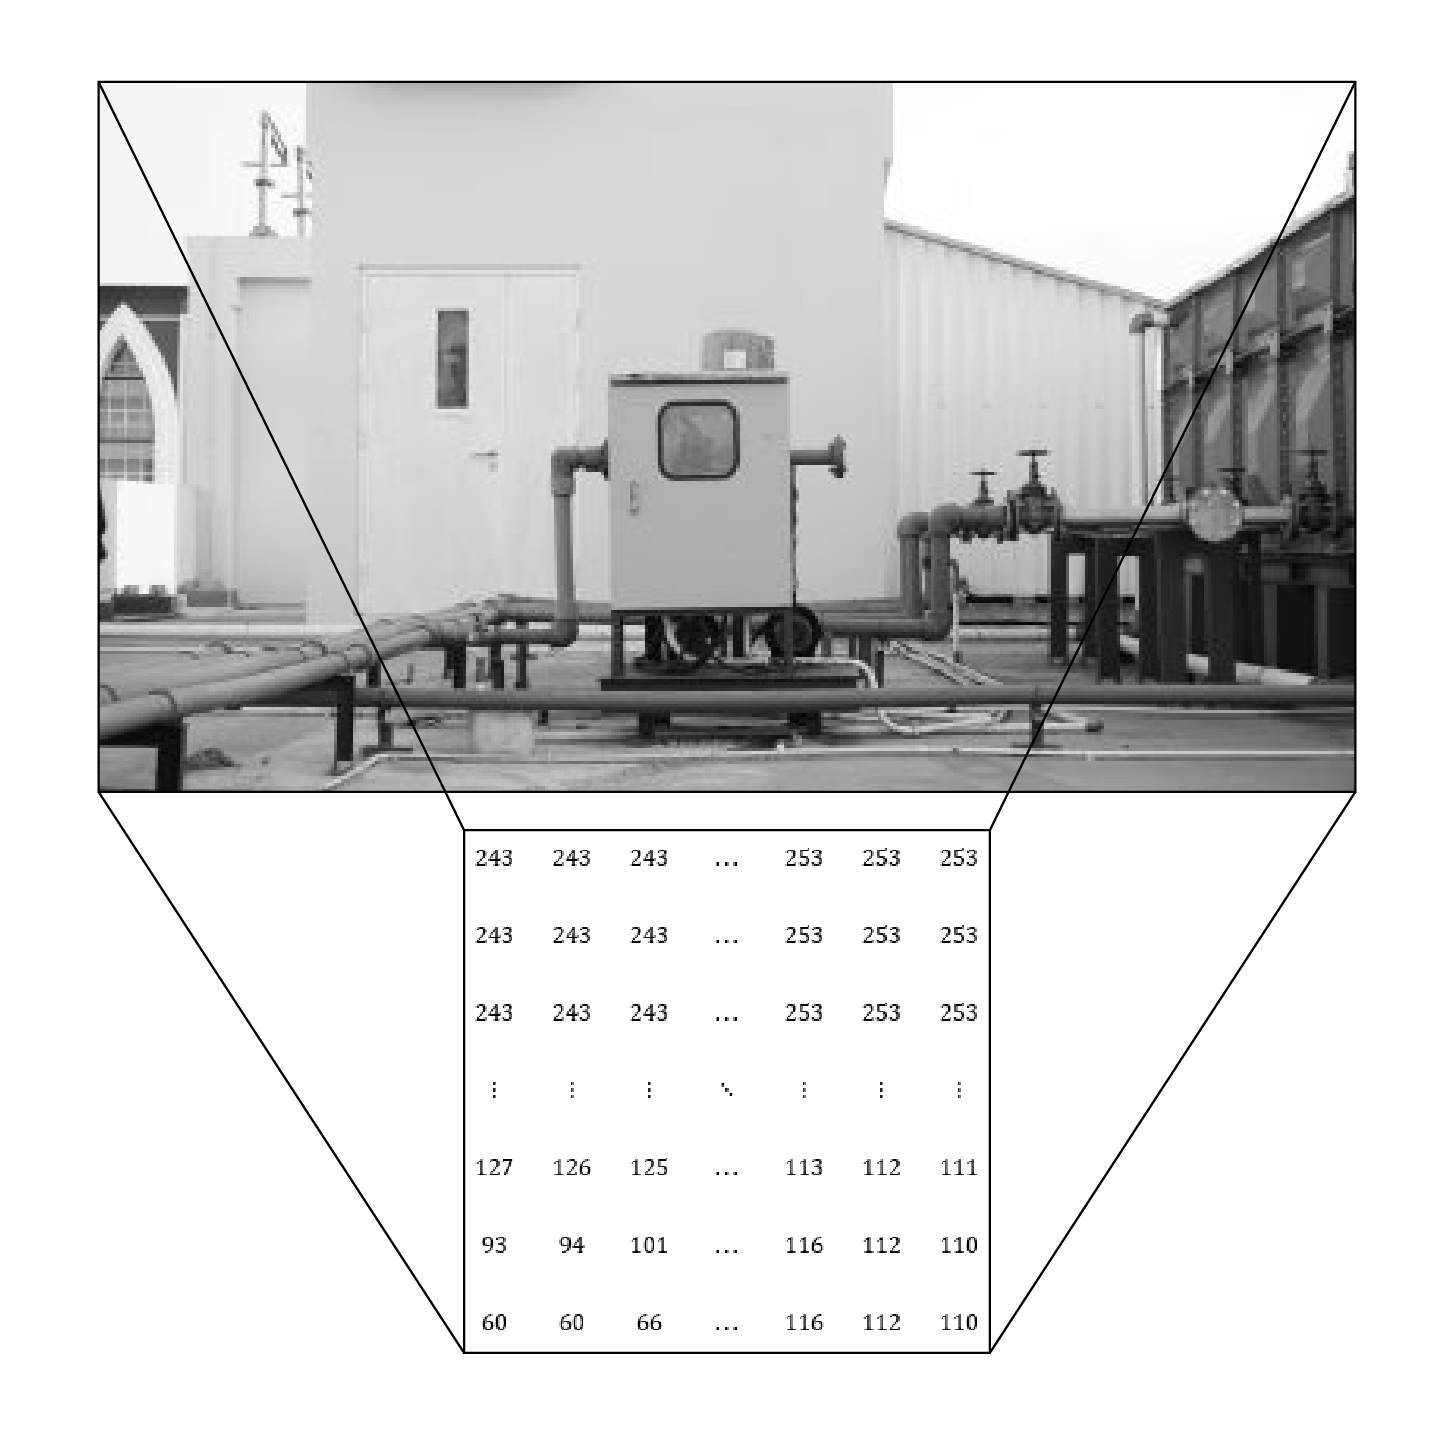
\includegraphics[width=8cm]{../img/Grayscale - Latex.png}
            \caption{Citra \textit{grayscale} beserta nilai pikselnya}
            \label{fig:grayscale}
            Sumber: \citep{Kusumanto2011}
        \end{center}
    \end{figure}

    \subsection{Citra Biner}
    Citra biner merupakan citra yang hanya memiliki dua nilai, yaitu $0$ atau $1$. Citra ini termasuk citra yang paling sederhana karena nilai $0$ pada suatu piksel citra biner menggambarkan warna hitam sedangkan nilai $1$ menggambarkan warna putih \citep{Kusumanto2011}. Contoh citra biner seperti terlihat pada Gambar \ref{fig:binary}.

    \begin{figure}[H]
        \begin{center}
            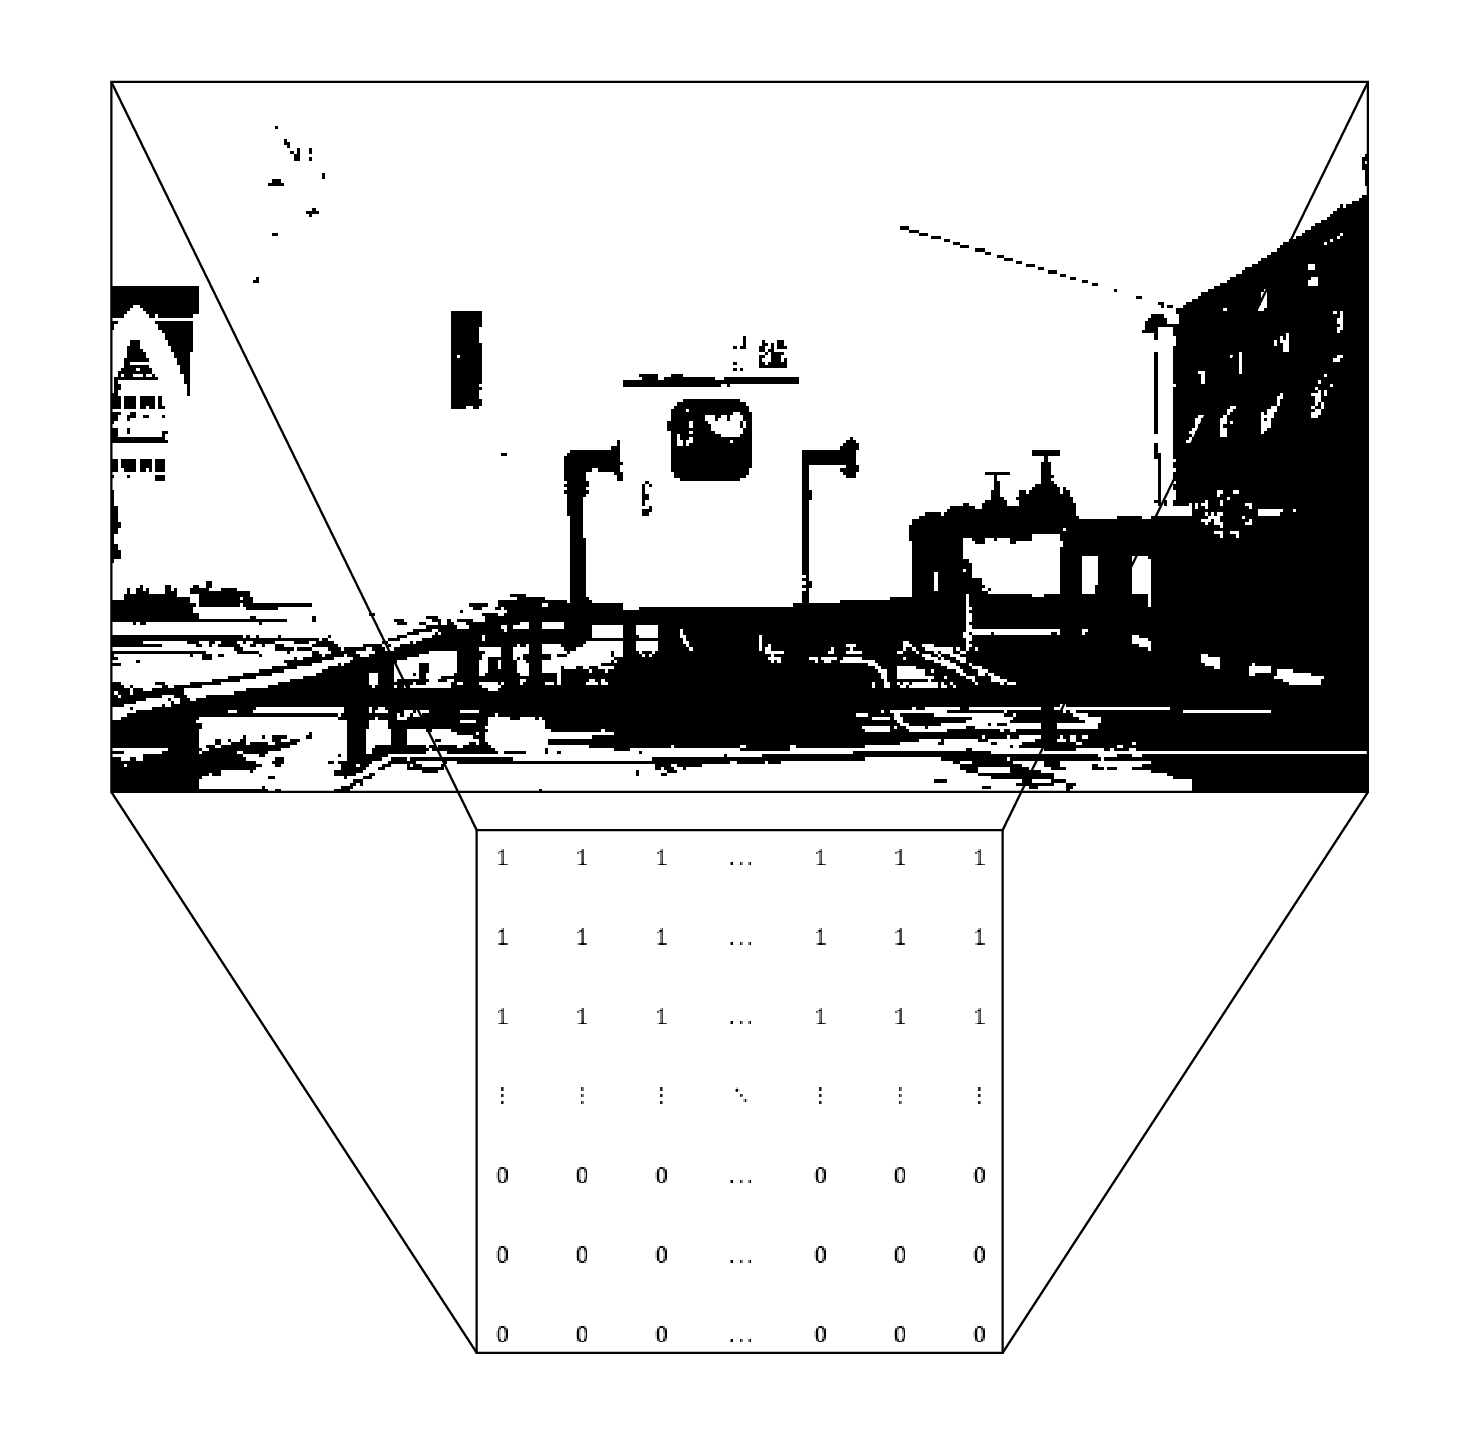
\includegraphics[width=8cm]{../img/Binary - Latex.png}
            \caption{Citra biner beserta nilai pikselnya}
            \label{fig:binary}
            Sumber: \citep{Kusumanto2011}
        \end{center}
    \end{figure}

    \subsection{Citra Dermoskopi}
    Dermoskopi menuju pada istilah dalam pemeriksaan kulit menggunakan mikroskop. Teknik ini merupakan teknik pencitraan kulit beresolusi tinggi yang memungkinkan visualisasi struktur kulit dengan mengurangi pantulan permukaan. Hal ini bertujuan untuk mengamati kulit dengan lebih detil dan mempermudah diagnosis kanker kulit. Sehingga, hasil dari teknik pencitraan kulit menggunakan mikroskop ini disebut sebagai citra dermoskopi \citep{Celebi2019}. Contoh citra dermoskopi seperti terlihat pada Gambar \ref{fig:dermoscopy}.

    \begin{figure}[H]
        \begin{center}
            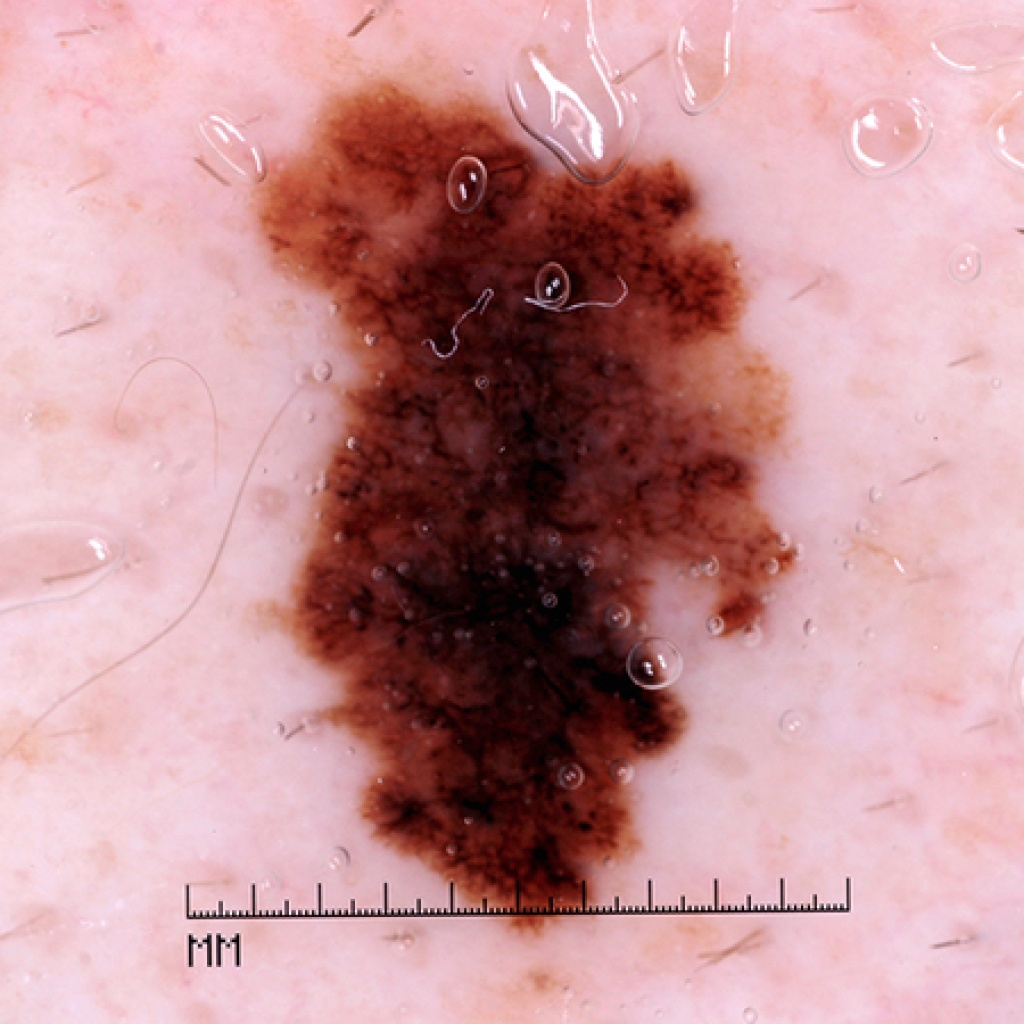
\includegraphics[width=4cm]{../img/Dermoscopy - Latex.jpg}
            \caption{Citra \textit{dermoscopy} yang mengandung kanker kulit \textit{melanoma}}
            \label{fig:dermoscopy}
            Sumber: \citep{Nersisson2021a}
        \end{center}
    \end{figure}

\section{\textit{Resize}}
Dalam citra digital, \textit{resize} atau penskalaan gambar merupakan proses rekontruksi citra untuk mengubah ukuran sebuah citra \citep{Morsy2018}. Pengubahan ukuran citra biasanya terjadi untuk menyamakan ukuran citra dan mengurangi waktu komputasi \citep{AhmedThaajwer2020a,Umamaheswari2018}. Contoh penskalaan gambar seperti terlihat pada Gambar \ref{fig:resize}.

\begin{figure}[H]
    \centering
    \begin{tabular}{cc}
        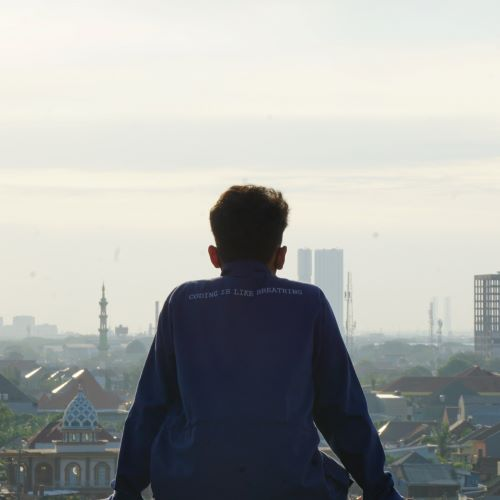
\includegraphics[width=4cm]{../img/Resize - Latex.JPG}
        &
        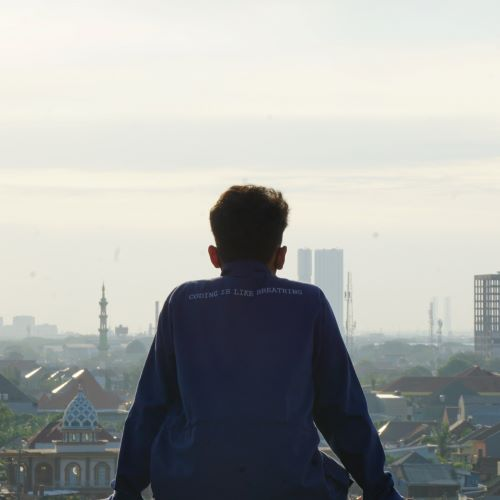
\includegraphics[width=2cm]{../img/Resize - Latex.JPG}\\
        (a) &(b)\\
    \end{tabular}
    \caption{(a) Citra sebelum diubah berukuran $500\times 500$ piksel (b) Citra setelah diubah berukuran $200\times 200$ piksel}
    \label{fig:resize}
    Sumber: \citep{Morsy2018}
\end{figure}

\section{Deteksi Objek}
Deteksi objek merupakan salah satu proses penting dalam \textit{computer vision} dengan mendeteksi sebuah objek pada sebuah citra dengan kelas tertentu, misalnya mobil, manusia, hewan secara spesifik, atau yang lainnya. Sebagai salah satu bagian penting dalam \textit{computer vision}, deteksi objek merupakan dasar dari beberapa tugas \textit{computer vision} seperti melacak objek, segmentasi objek, dan mengambil teks dalam gambar \citep{Zou2019}. Contoh deteksi objek seperti terlihat pada Gambar \ref{fig:obj-det}.

\begin{figure}[H]
    \begin{center}
        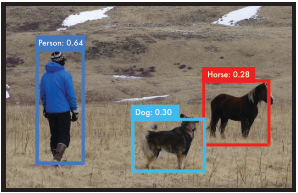
\includegraphics[width=8cm]{../img/Object Detection - Latex.png}
        \caption{YOLO dapat mendeteksi objek manusia, anjing, kuda}
        \label{fig:obj-det}
        Sumber: \citep{Redmon2016a}
    \end{center}
\end{figure}

\section{\textit{Convolutional Neural Networks} (CNN)}
CNN merupakan salah satu bagian dari deep learning dan pengembangan dari \textit{Multi Layer Perceptron} (MLP). CNN merupakan algoritma yang mirip dengan \textit{Artificial Neural Network} (ANN). Bahkan karena kemiripannya, strategi pengembangan ANN dapat diterapkan pada CNN. Data masukan pada CNN berupa matriks dari citra sehingga menghasilkan keluaran berupa skor atau bobot tertentu. Layer terakhir pada sebuah CNN mengandung loss function yang diasosiasikan dengan kelas tertentu. Pada umumnya, perbedaan ANN dan CNN terletak pada CNN yang lebih mengutamakan pengenalan pola pada sebuah citra. Hal ini dapat mengeluarkan fitur spesifik pada sebuah citra sehingga diolah pada arsitektur CNN.

Berdasarkan kemampuan CNN yang dapat mengolah data citra, neuron pada CNN terdiri atas neuron tiga dimensi. Neuron tersebut mengandung dimensi spasial dari data masukan, yaitu \textit{height}, \textit{width}, dan \textit{depth}. \textit{Depth} tidak mengacu pada jumlah layer pada jaringan, akan tetapi mengacu pada dimensi ketiga dari \textit{activation volume}. Neuron pada setiap layer hanya terkoneksi terhadap layer yang mendahuluinya. CNN terdiri dari tiga jenis layer, yaitu \textit{convolutional layer}, \textit{pooling layer}, dan \textit{fully-connected layers}. Arsitektur dasar pada CNN seperti terlihat pada Gambar \ref{fig:cnn}.

\begin{figure}[H]
    \begin{center}
        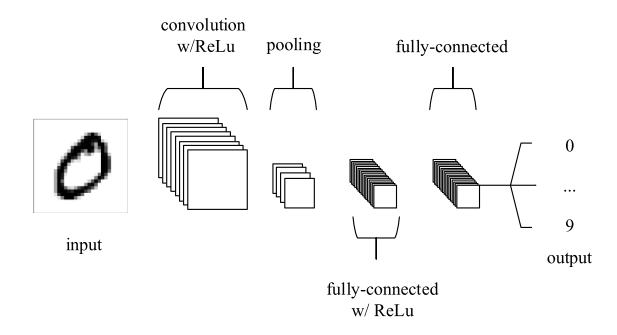
\includegraphics[width=12cm]{../img/CNN Basic - Latex.png}
        \caption{Arsitektur dasar dari CNN}
        \label{fig:cnn}
        Sumber: \citep{OShea2015}
    \end{center}
\end{figure}

\section{\textit{You Only Look Once version 7} (YOLO-v7)}
YOLO merupakan sebuah algoritma yang dapat digunakan untuk mendeteksi objek secara \textit{real time}. Algoritma ini bekerja dengan membagi citra ke dalam beberapa kotak sehingga YOLO memprediksi batas kotak pada sebuah objek. Hasil prediksi tersebut kemudian diklasifikasikan ke dalam kelas tertentu dengan memilih batas kotak yang memiliki nilai paling tinggi. YOLO merupakan algoritma deteksi objek berdasarkan \textit{Fully Connected Neural Network} (FCNN). Secara umum, terdapat tiga komponen utama pada YOLO, yaitu \textit{backbone}, \textit{neck}, dan \textit{head}. \textit{Backbone} melakukan ekstraksi fitur yang sangat esensial pada sebuah citra kemudian diteruskan ke \textit{neck}. Bagian \textit{neck} mengumpulkan \textit{feature map} yang diekstraksi dari \textit{backbone} dan membuat \textit{feature pyramid}. Pada akhirnya, \textit{head} melakukan deteksi untuk terakhir kalinya.

    \subsection{\textit{Convolutional Layer}}
    \textit{Convolutional Layer} merupakan layer utama dari CNN karena pada layer ini citra diolah dan dipelajari oleh CNN. \textit{Convolutional layer} menerapkan operasi konvolusi dengan tujuan mendapatkan fitur-fitur yang ada pada citra, seperti \textit{edge}, \textit{color}, \textit{shape}, dan fitur lainnya. Operasi konvolusi terjadi antara matriks dari data masukan, yaitu citra dan matriks kernel. Kernel merupakan matriks berisi nilai $-1$ atau $1$ dengan ukuran tertentu yang berguna untuk mendapatkan fitur dari citra sesuai dengan ukuran matriks kernel. Kernel memproses citra masukan dengan cara bergeser sebanyak \textit{stride} yang ditentukan. Hasil keluaran dari \textit{convolutional layer} berupa \textit{feature map} yang didapatkan dari sebuah citra masukan. Gambar \ref{fig:conv} menunjukkan representasi dari \textit{convolutional layer}.

    \begin{figure}[H]
        \begin{center}
            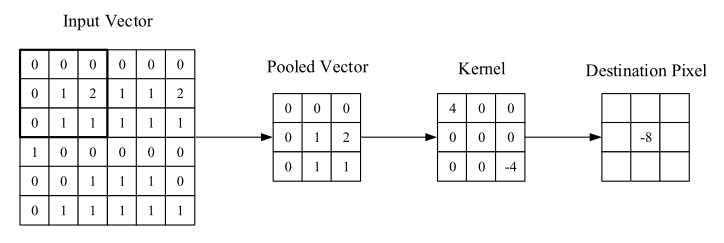
\includegraphics[width=12cm]{../img/CNN Convolutional Layer - Latex.png}
            \caption{Cara kerja kernel pada \textit{convolutional layer}}
            \label{fig:conv}
            Sumber: \citep{OShea2015}
        \end{center}
    \end{figure}

    \subsection{\textit{Pooling Layer}}
    \textit{Pooling layer} merupakan layer yang memproses \textit{feature map} dari \textit{convolutional layer}. Layer ini berfungsi untuk mengurangi volume pada setiap tumpukan \textit{feature map} tanpa menghilangkan informasi yang dibutuhkan. Terdapat beberapa jenis \textit{pooling layer} seperti, \textit{max pooling} dan \textit{average pooling}. \textit{Max pooling} mengambil nilai tertinggi pada \textit{feature map} dengan mempertimbangkan ukuran tertentu. Sedangkan \textit{average pooling} mengambil nilai rata-rata pada \textit{feature map} dengan mempertimbangkan ukuran tertentu. Proses \textit{max pooling} dan \textit{average pooling} seperti terlihat pada Gambar \ref{fig:pooling}.

    \begin{figure}[H]
        \centering
        \begin{tabular}{cc}
            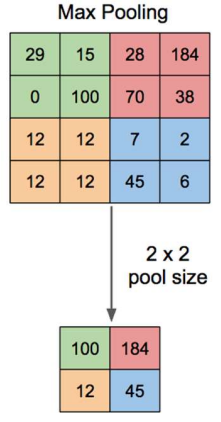
\includegraphics[width=3cm]{../img/CNN Max Pooling - Latex.PNG}
            &
            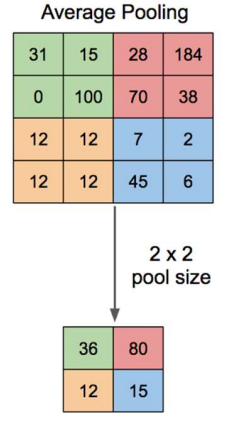
\includegraphics[width=3cm]{../img/CNN Average Pooling - Latex.PNG}\\
            (a) &(b)\\
        \end{tabular}
        \caption{Cara kerja \textit{pooling layer} (a) \textit{Max pooling}; (b) \textit{Average pooling}}
        \label{fig:pooling}
        Sumber: \citep{Yani2019}
    \end{figure}

    \subsection{\textit{Fully-Connected Layer}}
    \textit{Fully-Connected Layer} merupakan layer yang akan melakukan klasifikasi terhadap keluaran dari \textit{convolutional layer} dan \textit{pooling layer}. Matriks dengan jumlah n dimensi pada keluaran sebelumnya, diubah menjadi matriks dengan satu dimensi pada \textit{fully-connected layer} sebelum pada akhirnya dilakukan klasifikasi. Perhitungan pada \textit{fully-connected layer} seperti terlihat pada Persamaan \ref{eq:fcl}.
    \begin{align}
        y_j &= b_j + \sum_{i} w_{ij}x_i
        \label{eq:fcl}
    \end{align}

    $y$ merupakan keluaran dari \textit{fully-connected layer}, $b$ merupakan bias, $w$ merupakan bobot pada jaringan dengan ukuran $i\times j$ dengan $i$ yang merepresentasikan jumlah fitur dan $j$ yang merepresentasikan jumlah kelas, dan $x$ merupakan hasil keluaran dari layer sebelumnya.
	Pada dasarnya, \textit{fully-connected layer} selalu diisi dengan fungsi aktivasi \textit{softmax}. \textit{Softmax} merupakan fungsi aktivasi yang mengubah nilai angka atau log ke dalam probabilitas. Keluaran dari \textit{softmax} merupakan vektor dengan probabilitas pada setiap hasil yang mungkin. Secara matematis, \textit{softmax} dapat dituliskan seperti pada Persamaan \ref{eq:softmax}.
    \begin{align}
        S(y)_i &= \frac{e^{y_i}}{\sum_{j=1}^{n} e^{y_j}} 
        \label{eq:softmax}
    \end{align}

    $S(y)_i$ merupakan nilai probabilitas $y_i$, $n$ merupakan jumlah kelas, $y_i$ merupakan vektor masukan pada fungsi aktivasi \textit{softmax}. Hasil dari fungsi aktivasi \textit{softmax} berupa nilai antara $0$ sampai $1$ sehingga membuat distribusi probabilitas yang valid.

    \subsection{CSPDarknet53}
    CSPDarknet53 merupakan salah satu jenis CNN dan \textit{backbone} dari sebuah deteksi objek yang menggunakan arsitektur Darknet53 dengan \textit{Cross Stage Partial Network} (CSPNet). CSPDarknet53 terdiri dari \textit{based convolution layer} dan jaringan CSP. CSPDarknet53 menggunakan CSPNet untuk melakukan partisi \textit{feature map} pada \textit{based layer} menjadi dua bagian kemudian menggabungkannya secara \textit{cross-stage hierarchy}. Arsitektur CSP seperti terlihat pada Gambar \ref{fig:cspnet}.

    \begin{figure}[H]
        \centering
        \begin{tabular}{cc}
            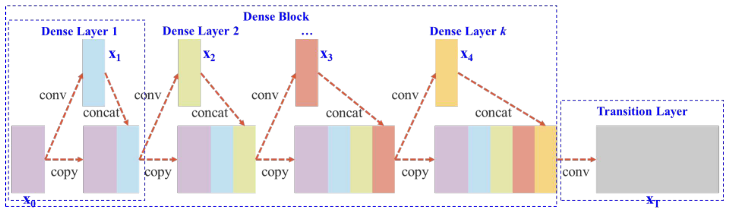
\includegraphics[width=7cm]{../img/DenseNet - Latex.PNG}
            &
            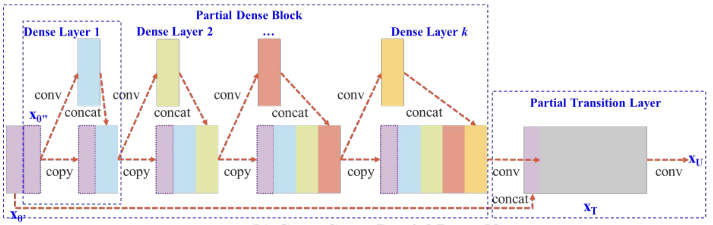
\includegraphics[width=7cm]{../img/CSP DenseNet - Latex.PNG}\\
            (a) &(b)\\
        \end{tabular}
        \caption{Modifikasi arsitektur DenseNet menjadi CSP DenseNet (a) DenseNet; (b) CSP DenseNet}
        \label{fig:cspnet}
        Sumber: \citep{Wang2020}
    \end{figure}

    Seperti terlihat pada Gambar \ref{fig:cspnet} (a), arsitektur DenseNet tidak ada pembagian \textit{feature map} pada \textit{based layer}. Sedangkan hasil modifikasi DenseNet menjadi CSP DenseNet membagi \textit{feature map} pada \textit{based layer} menjadi dua bagian seperti terlihat pada Gambar \ref{fig:cspnet} (b). Bagian pertama akan diteruskan ke dalam \textit{dense block} dan sebuah \textit{trainsition layer}. Sedangkan bagian lainnya akan dikombinasikan dengan \textit{transmitted feature map} untuk masuk ke tahap selanjutnya. Sehingga CSPNet dapat mengurangi waktu komputasi secara signifikan, meningkatkan waktu inferensi model, dan meningkatkan akurasi.

    \subsection{\textit{Spatial Pyramid Pooling} (SPP)}
    Pada arsitektur YOLOv1, YOLOv2, dan YOLOv3 \textit{feature map} diproses dengan cara memasuki \textit{max pooling layer} atau \textit{average pooling layer} kemudian diteruskan ke dalam \textit{fully-connected layers}. Sehingga YOLOv4 memodifikasi \textit{pooling layer} menjadi SPP agar YOLO menjadi lebih fleksibel untuk menerima input. SPP merupakan \textit{pooling layer} yang menyelesaikan masalah \textit{fixed-size} pada sebuah jaringan sehingga jaringan yang dibuat tidak perlu mengubah ukuran citra masukan pada tahap \textit{pre-processing} untuk menyamakan ukuran setiap citra masukan. Pada umumnya, SPP ditambahkan pada bagian akhir dari \textit{convolution layer}. Lapisan SPP menyatukan fitur dan menyamakan ukuran kemudian dimasukkan ke dalam \textit{fully-connected layers}. Dapat dikatakan bahwa SPP merupakan penyatuan informasi pada deep layer antara \textit{convolution layer} dan \textit{fully-connected layers} untuk menghindari proses pengubahan pada tahap \textit{pre-processing} \citep{He2014}. Proses SPP seperti terlihat pada Gambar \ref{fig:spatial-pyramid-pooling}.

    \begin{figure}[H]
        \begin{center}
            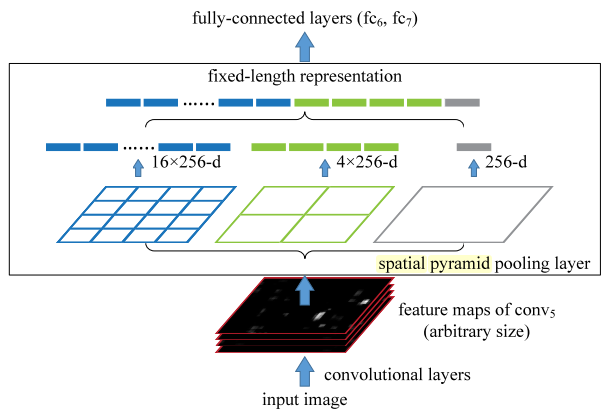
\includegraphics[width=8cm]{../img/Spatial Pyramid Pooling - Latex.png}
            \caption{Struktur SPP pada sebuah jaringan}
            \label{fig:spatial-pyramid-pooling}
            Sumber: \citep{He2014}
        \end{center}
    \end{figure}

    SPP mempertimbangkan informasi spasial dengan mengumpulkan respon dari filter pada setiap \textit{spatial bins}. Seperti terlihat pada Gambar \ref{fig:spatial-pyramid-pooling}, terdapat tiga level \textit{pooling} yang dilakukan. Keluaran \textit{feature map} memiliki $256$ filter dengan ukuran yang bergantung pada ukuran data masukan. Pada \textit{pooling} pertama, terdapat satu bin yang menutupi seluruh citra \textit{feature map}. Hasil dari \textit{pooling} ini berupa keluaran dengan ukuran $256$. Hal ini serupa dengan operasi \textit{global pooling}. \textit{Feature map} pada \textit{pooling} kedua memiliki $4$ bin sehingga menghasilkan keluaran dengan ukuran $4\times 256$. \textit{Pooling} ketiga memiliki $16$ bin dan menghasilkan keluaran dengan ukuran $16\times 256$. Hasil dari ketiga proses \textit{pooling} diratakan dan digabungkan pada sebuah vektor satu dimensi sehingga menghasilkan keluaran dengan ukuran tetap terlepas dari ukuran data masukan \citep{He2014}.

    \subsection{PANet}
    Pada arsitektur YOLO, PANet mulai digunakan pada YOLOv4 pada bagian \textit{neck} karena dapat meningkatkan kinerja model untuk proses deteksi objek. PANet merupakan jaringan yang dapat meningkatkan deteksi objek dengan menyediakan infomasi spasial secara akurat sehingga membantu lokalisasi piksel dan pembentukan \textit{mask} \citep{Liu2018}. Berikut ini merupakan beberapa fitur dari PANet:
    \begin{enumerate}
        \item \textit{Shorcut Connection}
        Semakin dalam sebuah jaringan, maka fitur yang didapatkan semakin kompleks dan resolusi spasial semakin berkurang. Sehingga \textit{pixel-level masks} tidak dapat diidentifikasi secara akurat. PANet melakukan augmentasi pada bagian \textit{top-down} dengan menambahkan bagian \textit{bottom-up} ke dalam bagian \textit{top-down} pada \textit{Feature Pyramid Network} (FPN) sehingga hal ini membentuk jalan pintas dari \textit{layer} bawah ke \textit{layer} atas. Proses \textit{shortcut connection} seperti terlihat pada Gambar \ref{fig:short-conn}.
        \begin{figure}[H]
            \begin{center}
                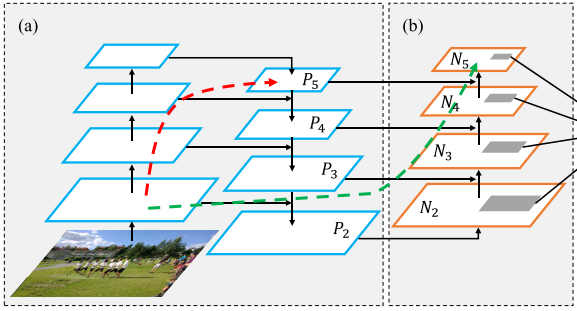
\includegraphics[width=8cm]{../img/PANet Shortcut Connection - Latex.png}
                \caption{Proses \textit{shortcut connection} pada PANet}
                \label{fig:short-conn}
                Sumber: \citep{Liu2018}
            \end{center}
        \end{figure}

        \item \textit{Adaptive Feature Pooling}
        Pada umumnya, jaringan menggunakan \textit{ROI Align Pooling} untuk memprediksi \textit{mask}. Akan tetapi, PANet menggunakan fitur dari semua \textit{layer} untuk memprediksi \textit{mask}. Sehingga jaringan dapat menentukan fitur yang paling berguna. \textit{Adaptive Feature Pooling} melakukan operasi \textit{ROI Align} pada setiap \textit{feature map} untuk mengekstrak fitur untuk objek. Hal ini menggunakan \textit{element-wise max fusion} untuk mendapatkan fitur baru. Proses \textit{Adaptive Feature Pooling} seperti terlihat pada Gambar \ref{fig:adaptive-feature-pooling}.
        \begin{figure}[H]
            \begin{center}
                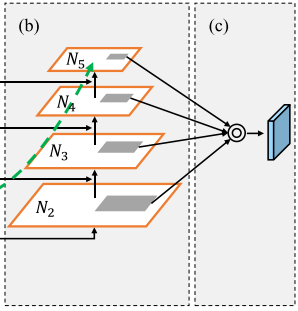
\includegraphics[width=4cm]{../img/PANet Adaptive Feature Pooling - Latex.png}
                \caption{Proses \textit{adaptive feature pooling} pada jaringan PANet}
                \label{fig:adaptive-feature-pooling}
                Sumber: \citep{Liu2018}
            \end{center}
        \end{figure}

        \item \textit{Fully-Connected Fusion}
        FCN menyediakan informasi spasial dan mengurangi jumlah parameter pada sebuah jaringan. Sedangkan, \textit{Fully-Connected Layers} dapat beradaptasi dengan informasi spasial. PANet menggunakan informasi dari keduanya untuk mendapatkan akurasi yang lebih tinggi dalam prediksi \textit{mask}. Proses \textit{Fully-Connected Fusion} seperti terlihat pada Gambar \ref{fig:fully-connected-fusion}.
        \begin{figure}[H]
            \begin{center}
                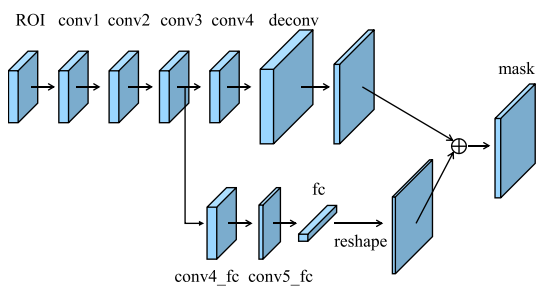
\includegraphics[width=8cm]{../img/PANet Fully Connected Fusion - Latex.png}
                \caption{Proses \textit{fully-connected fusion} pada jaringan PANet}
                \label{fig:fully-connected-fusion}
                Sumber: \citep{Liu2018}
            \end{center}
        \end{figure}

        Secara umum, PANet melakukan operasi adisi pada kedua \textit{layer} untuk memprediksi mask menggunakan \textit{Adaptive Feature Pooling}. Namun, YOLOv4 melakukan modifikasi pada PANet dengan mengubah operasi adisi menjadi operasi konkatenasi sehingga dapat meningkatkan akurasi. Arsitektur PANet yang telah dimodifikasi pada YOLOv4 seperti terlihat pada Gambar \ref{fig:panet}.

        \begin{figure}[H]
            \centering
            \begin{tabular}{cc}
                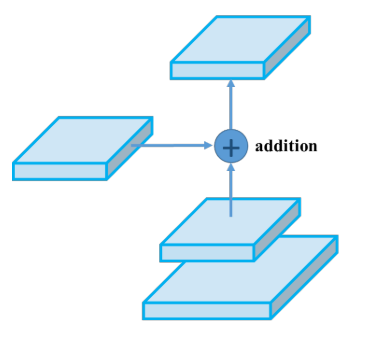
\includegraphics[width=4cm]{../img/PANet Original - Latex.PNG}
                &
                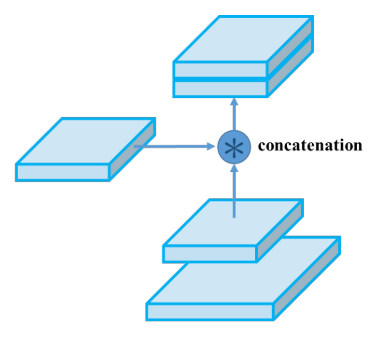
\includegraphics[width=4cm]{../img/PANet Modified - Latex.PNG}\\
                (a) &(b)\\
            \end{tabular}
            \caption{(a) Jaringan PANet Asli (b) Jaringan PANet modifikasi pada YOLO-v4}
            \label{fig:panet}
            Sumber: \citep{Bochkovskiy2020}
        \end{figure}

    \end{enumerate}

    \subsection{\textit{Extended Efficient Layer Aggregation Network} (E-ELAN)}
    E-ELAN merupakan salah satu blok komputasi pada sebuah \textit{backbone} di YOLO-v7. E-ELAN pada YOLO-v7 menggunakan \textit{expand}, \textit{shuffle}, dan \textit{merge cardinality} untuk mendapatkan kemampuan belajar secara terus menerus tanpa merusak \textit{original gradient path}. Pada dasarnya, E-ELAN membuat jaringan lebih baik dalam mempelajari data. E-ELAN merupakan modifikasi dari ELAN. Arsitektur E-ELAN seperti terlihat pada Gambar \ref{fig:e-elan}.

    \begin{figure}[H]
        \centering
        \begin{tabular}{cc}
            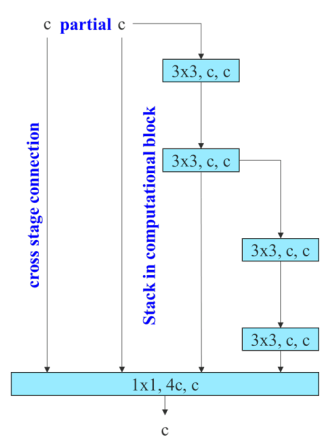
\includegraphics[width=4cm]{../img/ELAN - Latex.PNG}
            &
            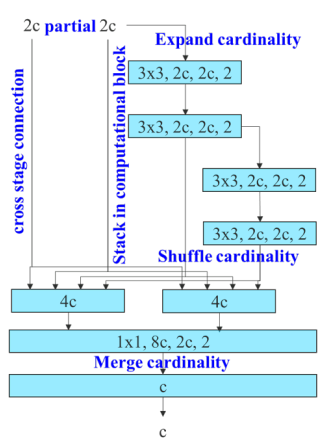
\includegraphics[width=4cm]{../img/E-ELAN - Latex.PNG}\\
            (a) &(b)\\
        \end{tabular}
        \caption{(a) Arsitektur ELAN; (b) Modifikasi ELAN menjadi E-ELAN}
        \label{fig:e-elan}
        Sumber: \citep{Wang2022}
    \end{figure}

    \subsection{\textit{Compound Scaling}}
    Setiap perangkat mempunyai keperluan yang berbeda-beda sehingga YOLO-v7 menyediakan fitur untuk mengubah ukuran model meskipun hal ini harus ditentukan di awal pelatihan model. Karena terdapat perangkat yang mengutamakan kecepatan atau akurasi. Dalam model scaling, terdapat beberapa parameter yang dipertimbangkan, yaitu \textit{resolution} (ukuran citra masukan), \textit{width} (jumlah saluran), \textit{depth} (jumlah layer), dan \textit{stage} (jumlah feature pyramid). Proses \textit{compound scaling} seperti terlihat pada Gambar \ref{fig:compound-scaling}.
    
    \begin{figure}[H]
        \centering
        \begin{tabular}{ccc}
            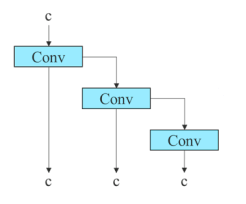
\includegraphics[width=3cm]{../img/Compound Scaling Concatenation-Based Model - Latex.PNG}
            &
            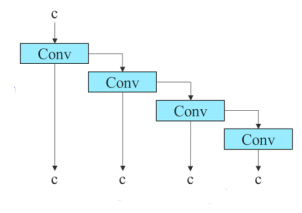
\includegraphics[width=3cm]{../img/Compound Scaling Scaled Up - Latex.PNG}
            &
            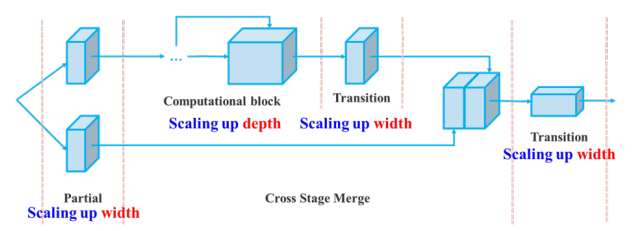
\includegraphics[width=6cm]{../img/Compound Scaling Up Depth and Width - Latex.PNG}\\
            (a) &(b) &(c)\\
        \end{tabular}
        \caption{Penskalaan model terhadap model \textit{concatenation-based} (a) Model \textit{concatention-based}; (b) \textit{Scaling-up} pada model \textit{concatenation-based}; (c) \textit{Compound scaling} pada \textit{concatenation-based} model}
        \label{fig:compound-scaling}
        Sumber: \citep{Wang2022}
    \end{figure}

\section{\textit{Confusion Matrix}}
\textit{Confusion matrix} merupakan salah satu metrik yang dapat menggambarkan performa dari sebuah algoritma klasifikasi. Secara matematis, \textit{confusion matrix} berupa matrix $C_{ij}$ yang berisi nilai integer yang tidak negatif dengan $i=1\cdots n,j=1\cdots n$ dimana $n$ merupakan jumlah kelas pada permasalahan klasifikasi. Elemen $C_{ij}$ merupakan hasil klasifikasi selama proses pengujian model. Jika $i=j$ maka kelas $i$ terklasifikasi dengan benar pada kelas $j$. Sehingga dapat dikatakan elemen pada diagonal utama matriks merupakan semua kelas yang terklasifikasi dengan benar. Sedangkan elemen tidak nol lainnya menandakan kesalahan klasifikasi \citep{Susmaga2004}. Setiap elemen pada \textit{confusion matrix} termasuk ke dalam beberapa kategori berikut \citep{Shultz2017}:
\begin{enumerate}
    \item \textit{True Positive} (TP) menunjukkan ketepatan model dalam mengklasifikasikan kelas positif sebagai kelas positif.
    \item \textit{False Positive} (FP) menunjukkan ketepatan model dalam mengklasifikasikan kelas positif sebagai kelas negatif.
    \item \textit{True Negative} (TN) menunjukkan ketepatan model dalam mengklasifikasikan kelas negatif sebagai kelas negatif.
    \item \textit{False Negative} (FN) menunjukkan ketepatan model dalam mengklasifikasikan kelas negatif sebagai kelas positif.
\end{enumerate}

Sehingga \textit{confusion matrix} dapat digambarkan ke dalam sebuah tabel seperti terlihat pada Tabel \ref{tab:conf-mat}. Pada Tabel \ref{tab:conf-mat} terdapat $1\cdots n$ kelas. Baris dan kolom pada Tabel \ref{tab:conf-mat} berturut-turut merepresentasikan data aktual dan hasil klasifikasi.

\begin{table}[H]
    \caption{\textit{Confusion matrix}}
    \centering
    \begin{tabular}{|c|c|c|c|c|}
        \hline
        \           &$1$        &$2$        &$\cdots$   &$n$\\
        \hline
        $1$         &$C_{11}$   &$FN$       &$\cdots$   &$C_{1n}$\\
        \hline
        $2$         &$FP$       &$TP$       &$\cdots$   &$FP$\\
        \hline
        $\vdots$    &$\vdots$   &$\vdots$   &$\ddots$   &$\vdots$\\
        \hline
        $n$         &$C_{n1}$   &$FN$       &$\cdots$   &$C_{nn}$\\
        \hline
    \end{tabular}

    \label{tab:conf-mat}
    Sumber: \citep{Shultz2017}
\end{table}

\section{\textit{Intersection over Union} (IoU)}
IoU merupakan indikasi untuk mengetahui seberapa tepat prediksi kotak pembatas ke terhadap objek yang ada pada citra. Semakin tinggi nilai IoU menandakan semakin baik prediksi kotak pembatas oleh model deteksi objek. Kondisi IoU seperti terlihat pada Gambar \ref{fig:iou-cond} (a) dimana $(x_1, y_1)$ dan $(x_2, y_2)$ merupakan koordinat kotak pembatas data aktual sedangkan $(x_3, y_3)$ dan $(x_4, y_4)$ merupakan koordinat kotak pembatas hasil prediksi.

\begin{figure}[H]
    \centering
    \begin{tabular}{ccc}
        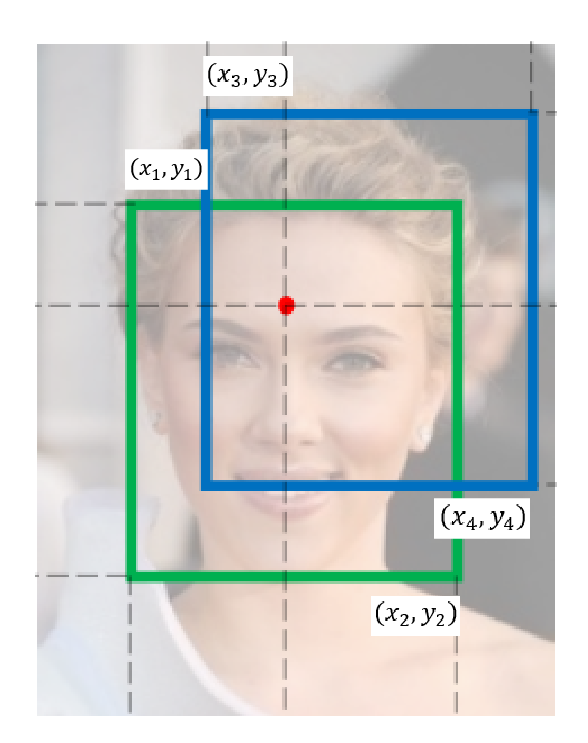
\includegraphics[width=3cm]{../img/IoU Bounding Box - Latex.png}
        &
        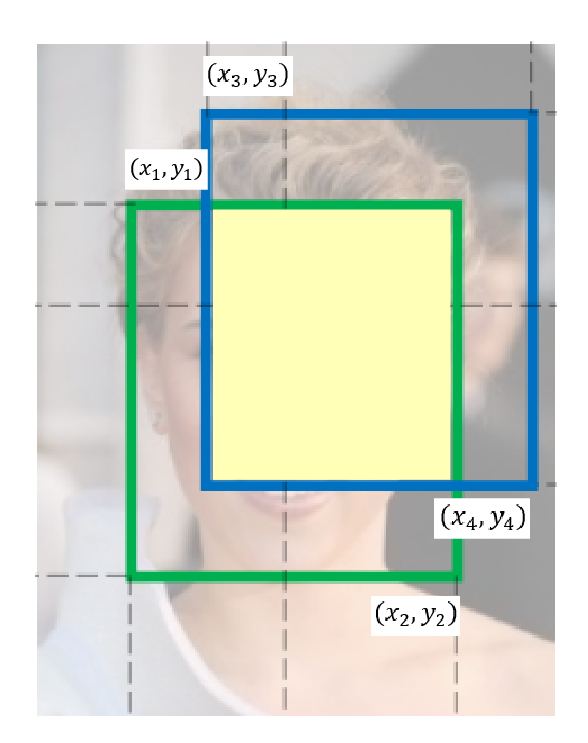
\includegraphics[width=3cm]{../img/IoU Overlapped Area - Latex.png}
        &
        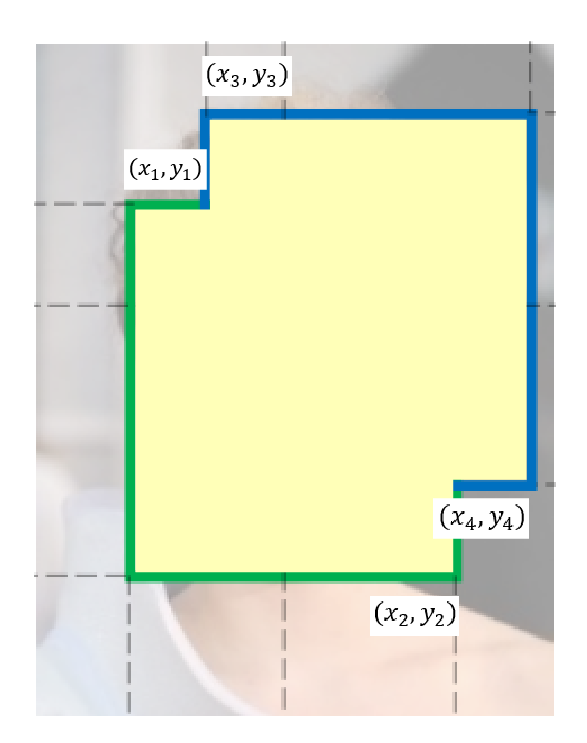
\includegraphics[width=3cm]{../img/IoU Union Area - Latex.png}\\
        (a) &(b) &(c)\\
    \end{tabular}
    \caption{Menunjukkan kondisi kotak pembatas (a) IoU; (b) \textit{Overlapped area}; (c) \textit{Union area}}
    \label{fig:iou-cond}
\end{figure}

Dari kedua kotak pembatas tersebut didapatkan dua bagian, yaitu \textit{overlap area} dan \textit{union area}. \textit{Overlap area} merupakan bagian tumpang tindih antara kotak pembatas data aktual dan kotak pembatas hasil prediksi. Sedangkan \textit{union area} merupakan gabungan antara kedua kotak pembatas. \textit{Overlap area} dan \textit{union area} seperti terlihat pada Gambar \ref{fig:iou-cond}. Pembagian antara \textit{overlap area} dengan \textit{union area} menghasilkan nilai IoU seperti pada Persamaan \ref{eq:iou}. Perhitungan \textit{overlap area} dan \textit{union area} seperti terlihat pada Persamaan \ref{eq:oa} dan \ref{eq:ua}. Nilai $x_a1, x_a2, y_a1, y_a2$ pada perhitungan tersebut didapatkan seperti pada Persamaan \ref{eq:xa1} - \ref{eq:ya2}.
\begin{align}
    \label{eq:xa1}
    x_{a1} &= max(x_1, x_3)\\
    \label{eq:xa2}
    x_{a2} &= max(x_2, x_4)\\
    \label{eq:ya1}
    y_{a1} &= max(y_1, y_3)\\
    \label{eq:ya2}
    y_{a2} &= max(y_2, y_4)\\
    \label{eq:oa}
    OA     &= (x_{a2}-x_{a1}\ast (y_{a2}-y_{a1}))\\
    \label{eq:ua}
    UA     &= (x_2-x_1)\ast (y_2-y_1) + (x_4-x_3)\ast (y_4-y_3) - OA\\
    \label{eq:iou}
    IoU    &= \frac{OA}{UA}
\end{align}

Dalam menentukan nilai IoU, sangat penting untuk memperhatikan ambang batas IoU. Karena hal ini akan menentukan kategori klasifikasi seperti pada Gambar \ref{fig:iou-cat}. Jika ambang batas IoU adalah $0.5$ maka Gambar \ref{fig:iou-cat} (a) termasuk ke dalam FP, Gambar \ref{fig:iou-cat} (b) dan (c) termasuk ke dalam TP. Sedangkan kondisi kotak pembatas data aktual dan kotak pembatas hasil prediksi tidak beririsan sama sekali dikategorikan sebagai FN.

\begin{figure}[H]
    \centering
    \begin{tabular}{ccc}
        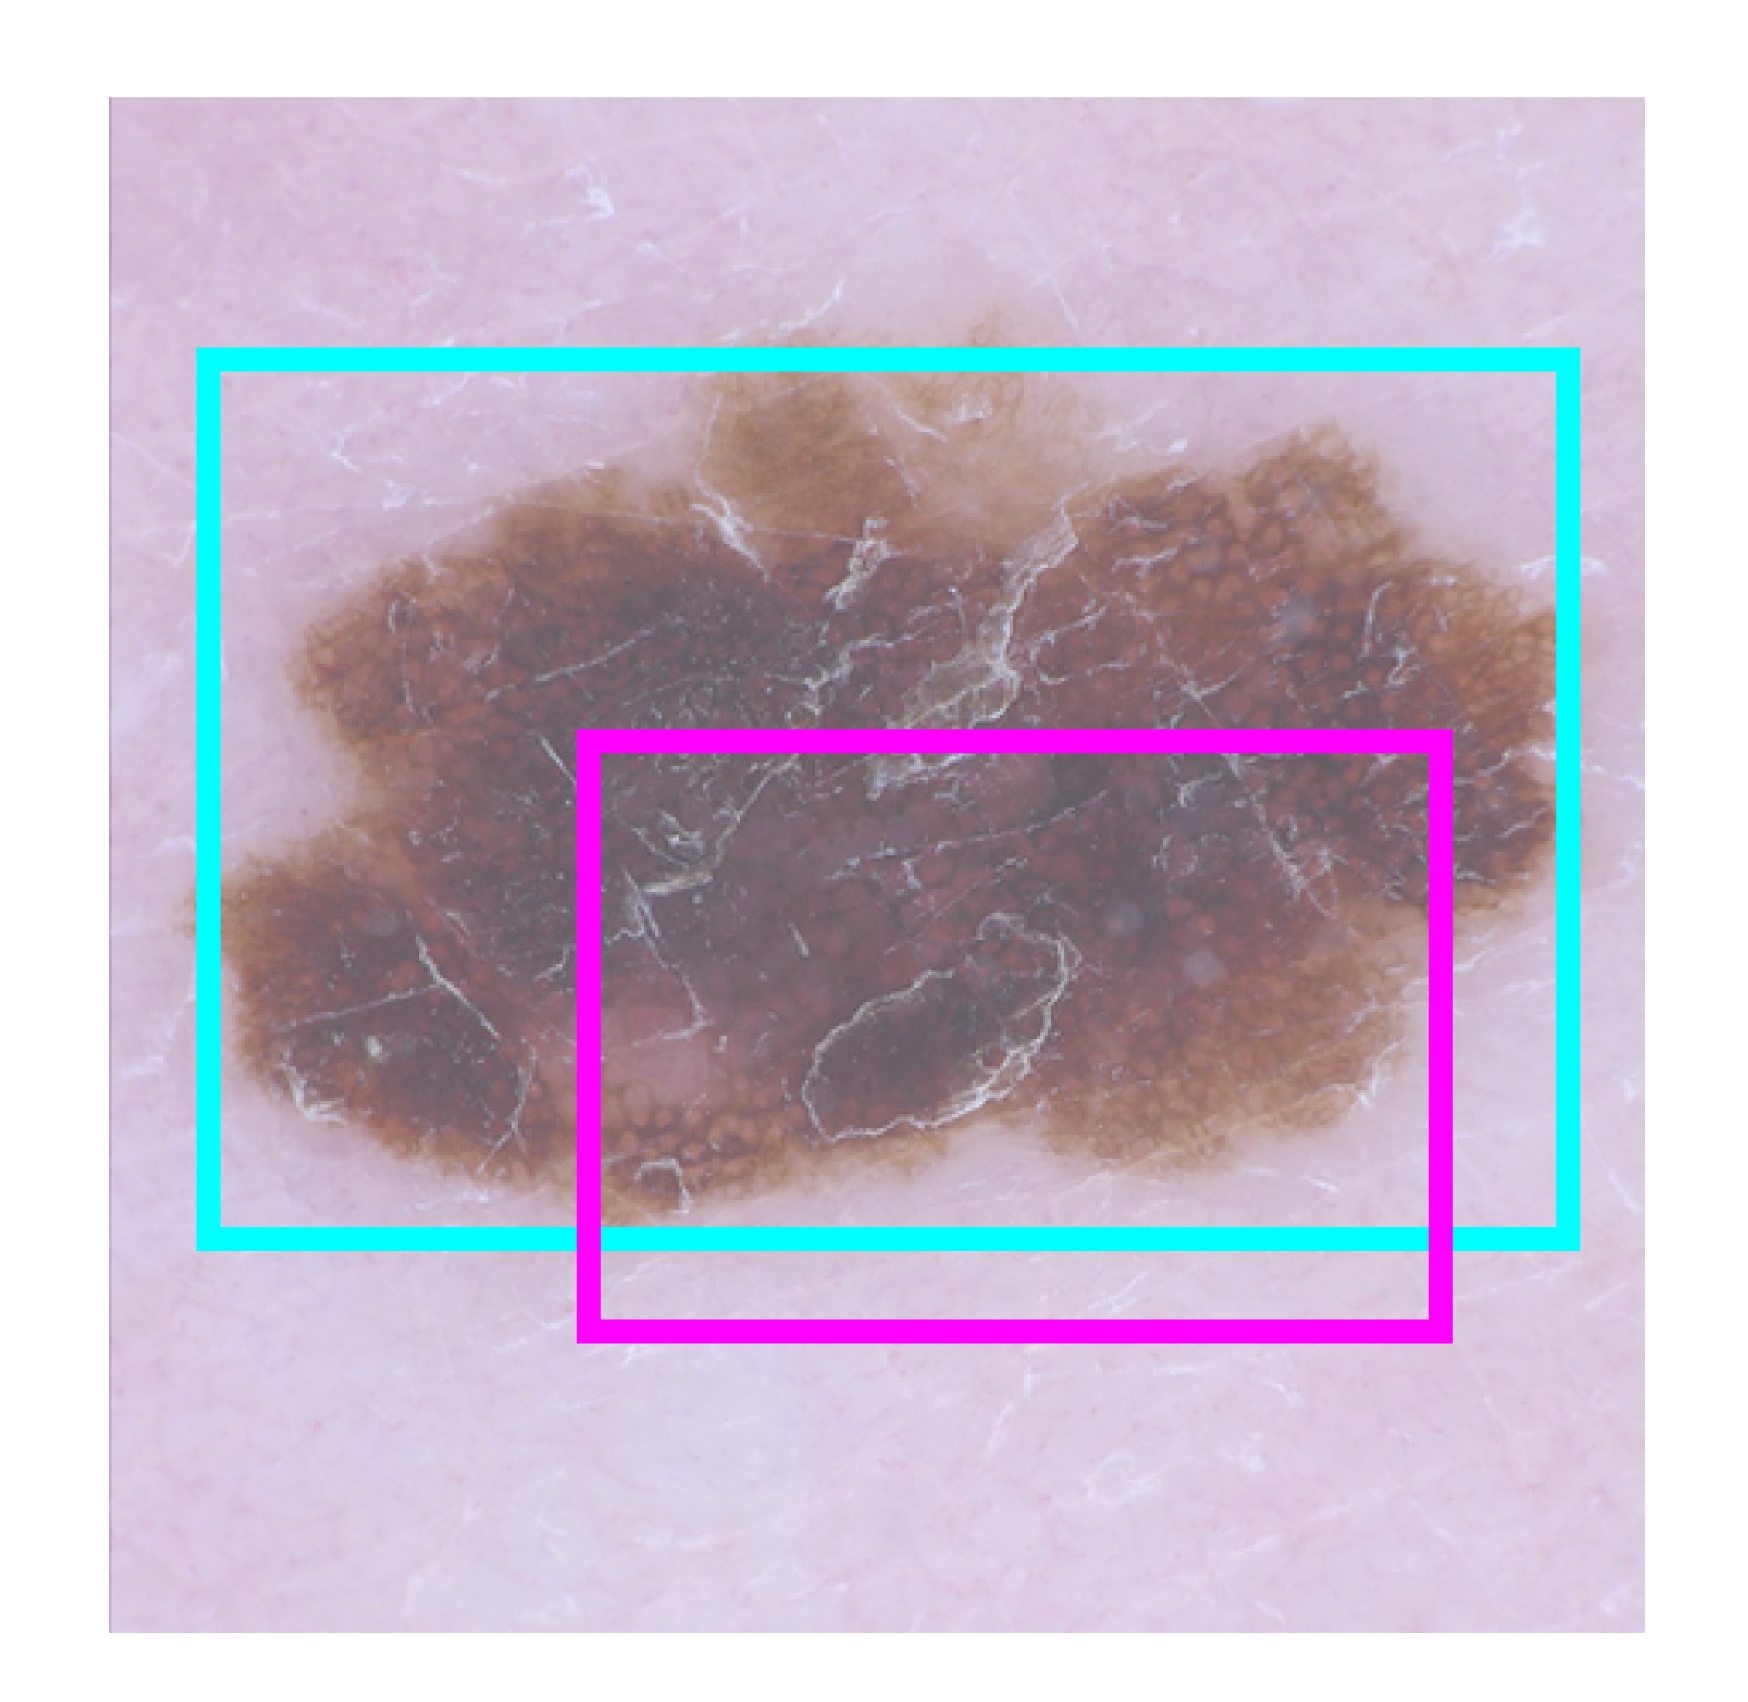
\includegraphics[width=2cm]{../img/IoU Poor - Latex.PNG}
        &
        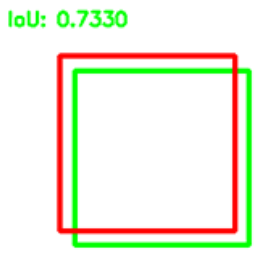
\includegraphics[width=2cm]{../img/IoU Good - Latex.PNG}
        &
        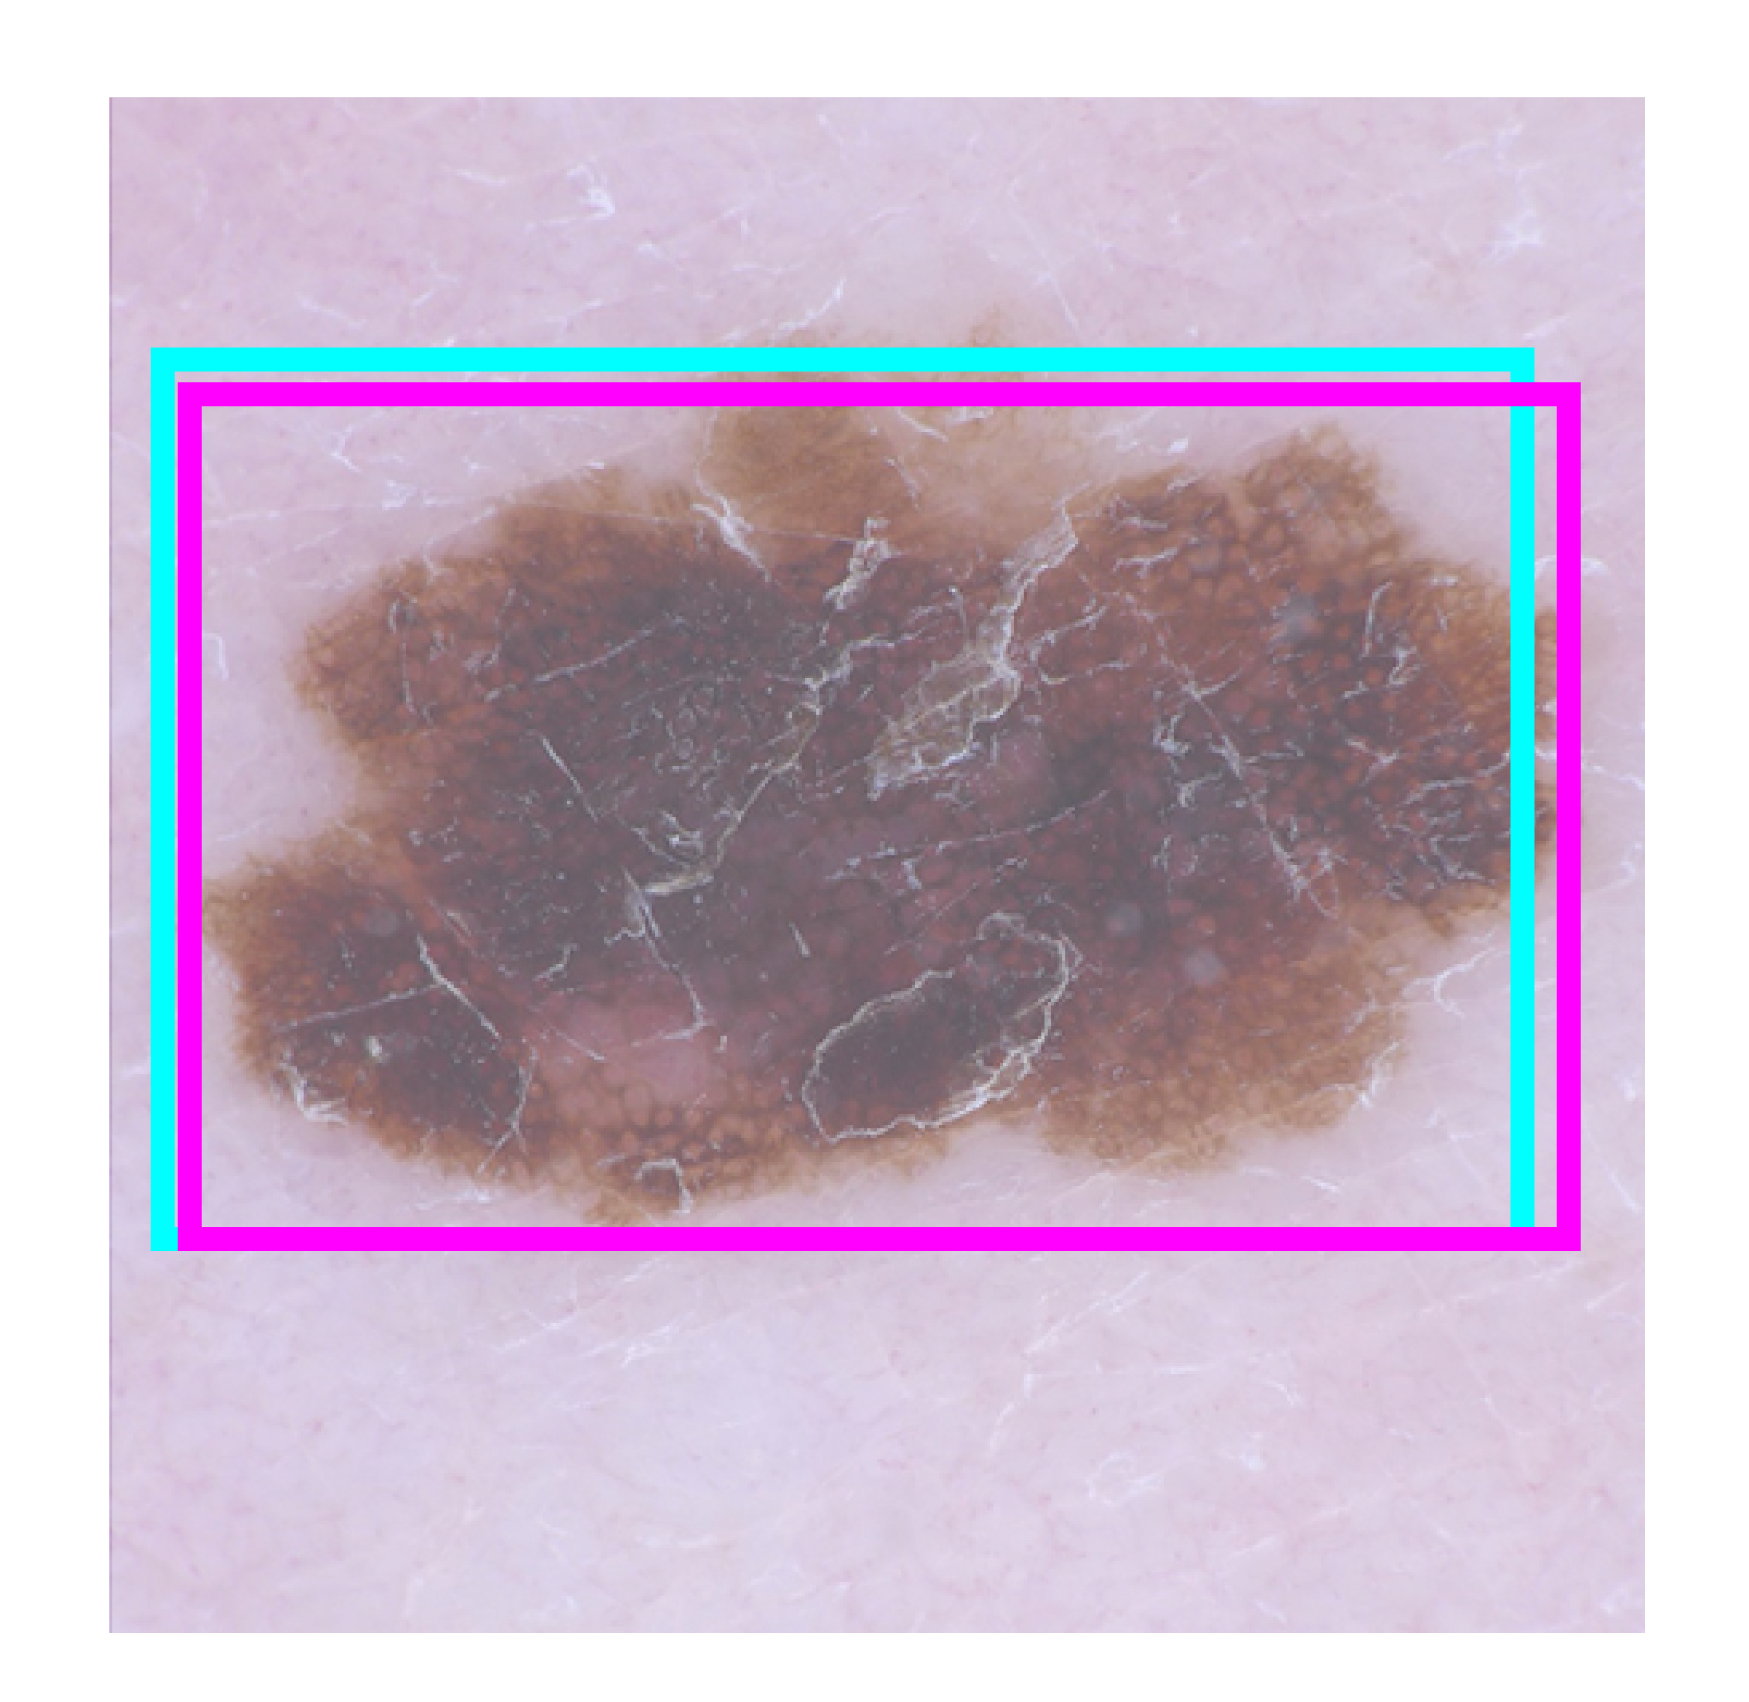
\includegraphics[width=2cm]{../img/IoU Excellent - Latex.PNG}\\
        (a) &(b) &(c)\\
    \end{tabular}
    \caption{Menunjukkan kondisi nilai IoU (a) Nilai IoU kurang baik; (b) Nilai IoU baik; (c) Nilai IoU sangat baik}
    \label{fig:iou-cat}
    Sumber: \citep{Cowton2019}
\end{figure}

\section{\textit{mean Average Precision} (mAP)}
mAP merupakan salah satu metode evaluasi model terutama pada model deteksi objek, seperti Fast R-CNN, MobileNet SSD, dan YOLO. Semakin baik model deteksi objek maka semakin tinggi nilai mAP. mAP menghitung rata-rata \textit{Average Precision} (AP) per kelas seperti terlihat pada Persamaan \ref{eq:map}. AP merupakan perhitungan \textit{precision} dan \textit{recall} pada setiap kelas seperti terlihat pada Persamaan \ref{eq:ap}. \textit{Precision} merupakan rasio antara kelas positif yang diprediksi dengan benar terhadap total data yang diklasifikasikan sebagai kelas positif. \textit{Recall} merupakan rasio antara kelas positif yang diprediksi dengan benar terhadap seluruh data positif. Perhitungan \textit{precision} dan \textit{recall} seperti terlihat pada Persamaan \ref{eq:precision} dan \ref{eq:recall} dimana $P$ dan $R$ merupakan \textit{precision} dan \textit{recall} \citep{Shultz2017}.
\begin{align}
    \label{eq:precision}
    P &= \frac{TP}{TP+FP}\\
    \label{eq:recall}
    R &= \frac{TP}{TP+FN}\\
    \label{eq:ap}
    AP &= \sum_{i=0}^{n-1} (R_i+R_{i+1})\ast P(i)\\
    \label{eq:map}
    mAP &= \frac{1}{n}\sum_{i=1}^{n} AP_i
\end{align}




    \chapter{METODE PENELITIAN}

\section{Jenis Penelitian}
Penelitian ini melakukan deteksi objek pada data citra dermoskopi menggunakan metode YOLO-v7. Berdasarkan hal tersebut, penelitian ini data numerik yang terdiri dari matriks dan nilai intensitas piksel sehingga penelitian ini termasuk ke dalam penelitian kuantitatif. Maka dari itu, pada penelitian ini terdapat perhitungan dan analisis terkait dengan data dan metode yang digunakan untuk mendeteksi kanker kulit pada citra dermoskopi.

\section{Jenis dan Sumber Data}
Penelitian ini menggunakan dataset yang berasal dari \textit{ISIC 2019 Challenge}. Dataset \textit{ISIC 2019 Challenge} memiliki 8 jenis kanker kulit, yaitu \textit{Actinic Keratosis}, \textit{Melanoma}, \textit{Squamous Cell Carcinoma}, \textit{Basal Cell Carcinoma}, \textit{Nevus}, \textit{Dermatofibroma}, \textit{Benign Keratosis Lesion}, dan \textit{Vascular Lesion}. Terdapat ribuan data citra kanker kulit, akan tetapi dengan mempertimbangkan perangkat yang digunakan untuk pembentukan model, penelitian ini menggunakan 200 citra pada tiap kelas sehingga terdapat 1600 data citra yang digunakan pada penelitian ini untuk pembentukan model. Sampel citra masing-masing jenis kanker kulit seperti terlihat pada Gambar \ref{fig:dataset}.

\begin{figure}[H]
    \centering
    \begin{tabular}{cccc}
        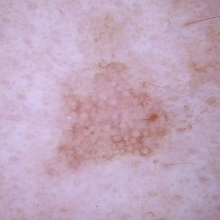
\includegraphics[width=2cm]{../img/Dataset - AK.png}
        &
        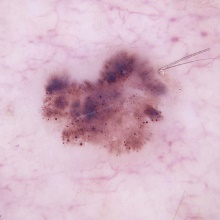
\includegraphics[width=2cm]{../img/Dataset - BCC.png}
        &
        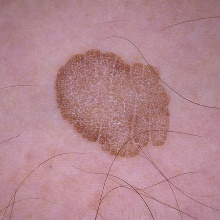
\includegraphics[width=2cm]{../img/Dataset - BKL.png}
        &
        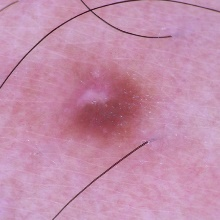
\includegraphics[width=2cm]{../img/Dataset - DF.png}\\
        (a) &(b) &(c) &(d)\\
        \  &\  &\  &\ \\
        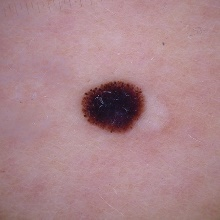
\includegraphics[width=2cm]{../img/Dataset - MEL.png}
        &
        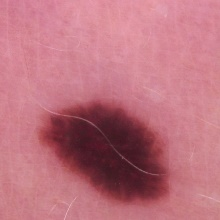
\includegraphics[width=2cm]{../img/Dataset - NV.png}
        &
        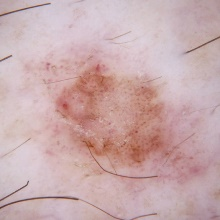
\includegraphics[width=2cm]{../img/Dataset - SCC.png}
        &
        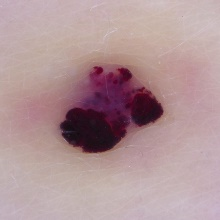
\includegraphics[width=2cm]{../img/Dataset - VASC.png}\\
        (e) &(f) &(g) &(h)\\
    \end{tabular}
    \caption{Dataset citra dermoskopi kanker kulit (a) AK; (b) BCC; (c) BKL; (d) DF; (e) MEL; (f) NV; (g) SCC; (h) VASC;}
    \label{fig:dataset}
\end{figure}

\section{Kerangka Penelitian}
Tahapan dalam melakukan deteksi kanker kulit berdasarkan citra dermoskopi menggunakan YOLO-v7 pada penelitian ini seperti terlihat pada Gambar \ref{fig:flowchart}.

\begin{figure}[H]
    \begin{center}
        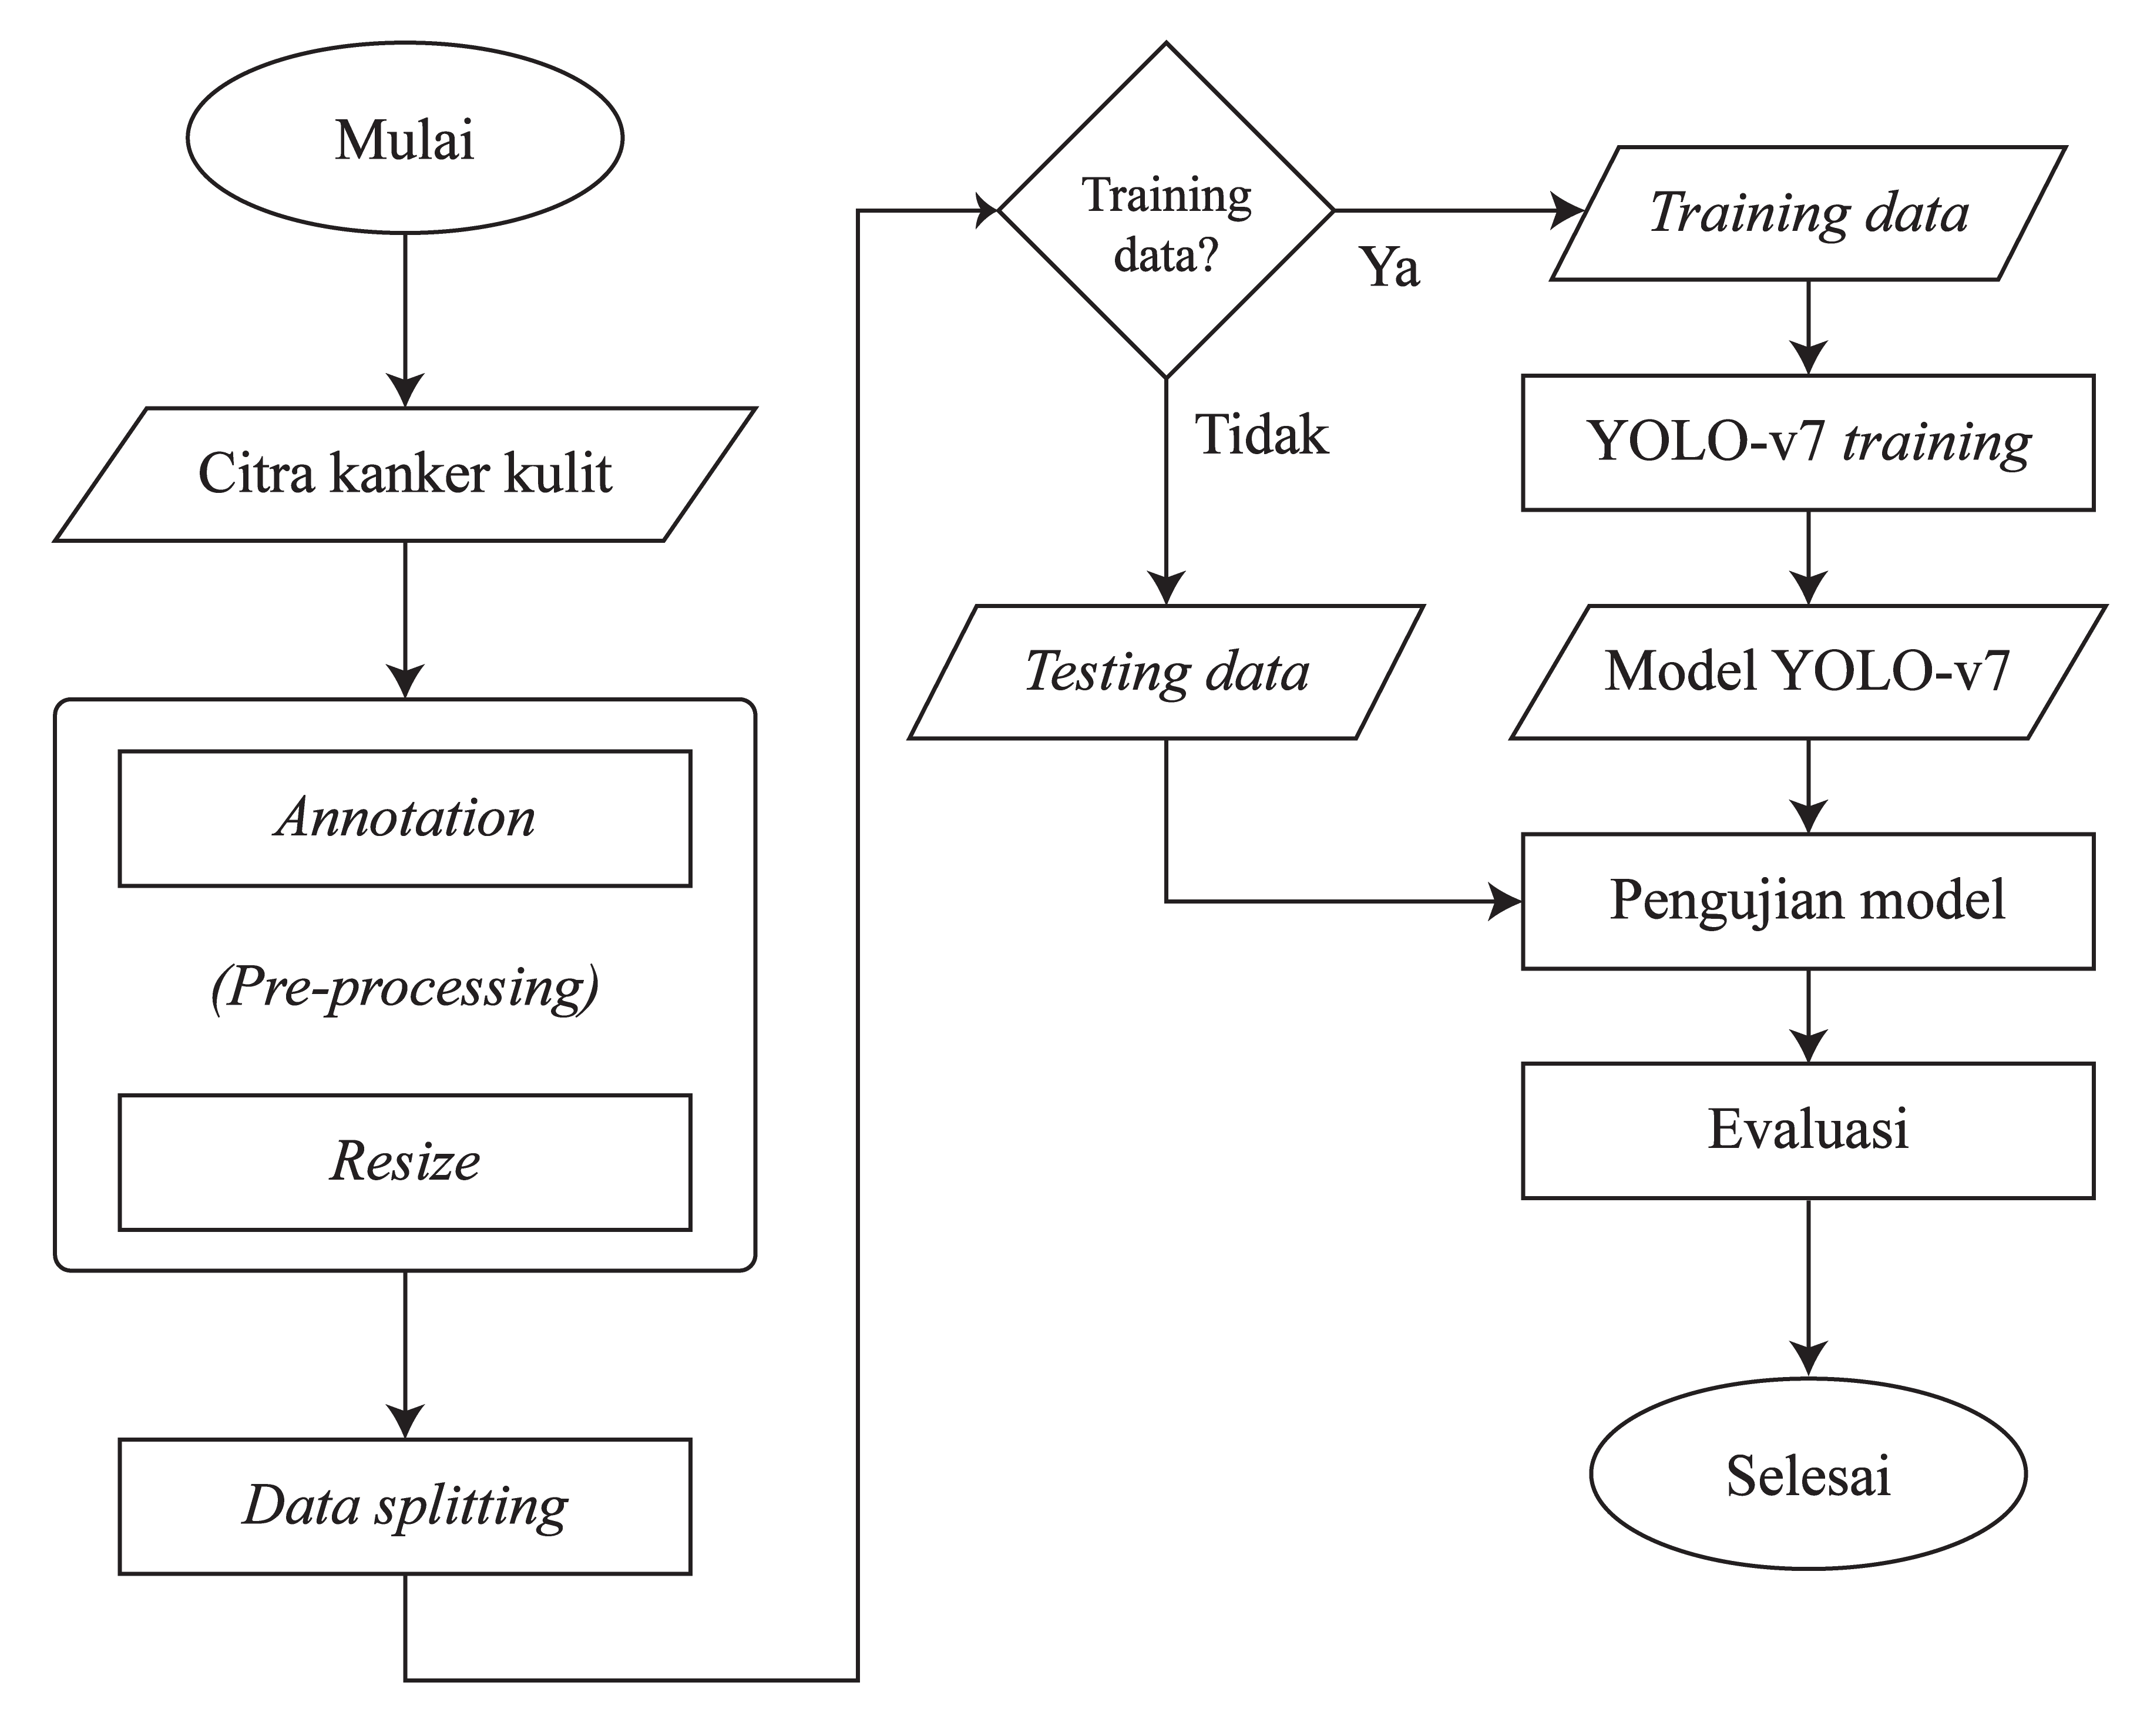
\includegraphics[width=13cm]{../img/Flowchart.png}
        \caption{Diagram alir pada penelitian ini}
        \label{fig:flowchart}
    \end{center}
\end{figure}

Penelitian ini terdiri dari beberapa proses sebagai berikut:
\begin{enumerate}
    \item Tahap \textit{pre-processing} terdiri dari \textit{annotation} dan \textit{resize}. \textit{Annotation} merupakan pemberian kotak pembatas sebuah objek pada sebuah citra. Hal ini dilakukan satu per satu sesuai dengan label yang diberikan dari penyedia dataset, yaitu \textit{ISIC 2019 Challenge}. \textit{Resize} merupakan pengubahan ukuran piksel pada sebuah citra, sehingga penelitian ini melakukan \textit{resize} citra masukan menjadi ukuran $640\times 640$. Rumus \textit{resize} seperti terlihat pada \ref{eq:resize}. Proses \textit{annotation} dan \textit{resize} seperti terlihat pada Gambar \ref{fig:preprocessing}.
    \begin{figure}[H]
        \centering
        \begin{tabular}{ccc}
            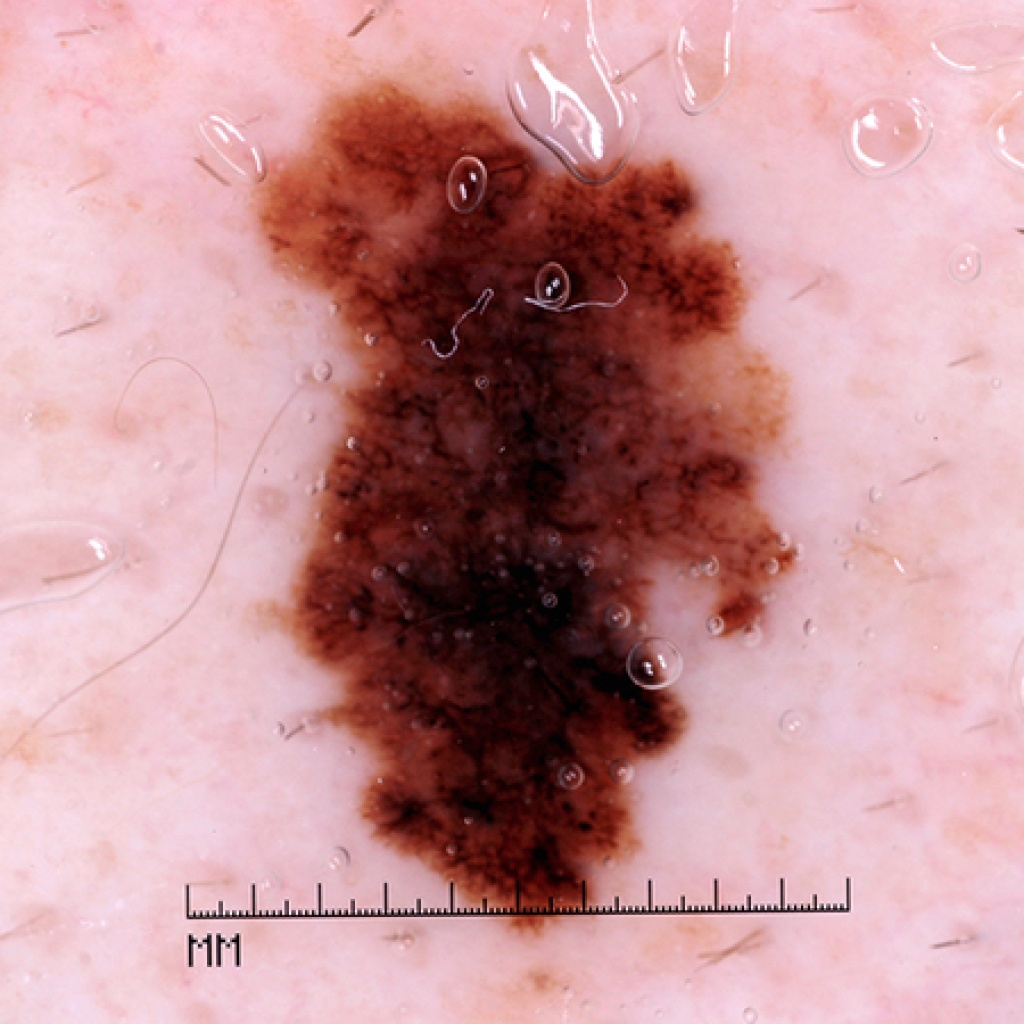
\includegraphics[width=2cm]{../img/Dermoscopy - Latex.jpg}
            &
            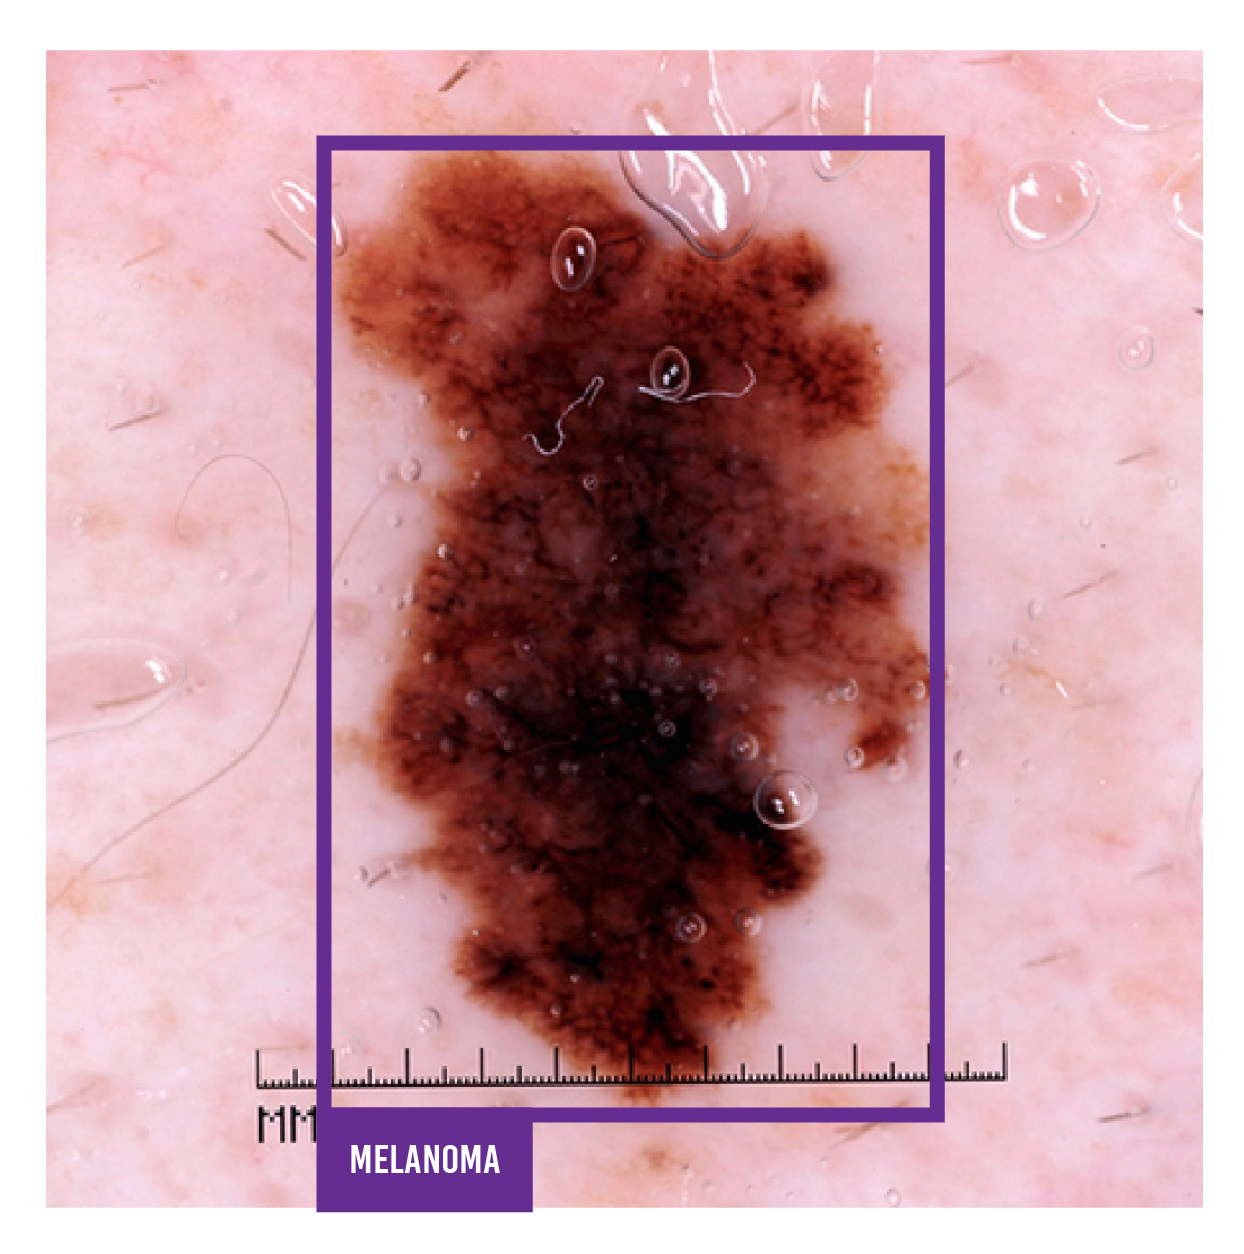
\includegraphics[width=2cm]{../img/Annotation - Latex.png}
            &
            \includegraphics[width=1.5cm]{../img/Annotation - Latex.png}\\
            (a) &(b) &(c)\\
        \end{tabular}
        \caption{Tahap \textit{pre-processing} (a) Citra asli; (b) Citra setelah menerapkan \textit{annotation}; (c) Citra setelah menerapkan \textit{resize}}
        \label{fig:preprocessing}
    \end{figure}

    \item \textit{Data splitting} merupakan tahap pembagian data. Penelitian ini membagi data menjadi tiga, yaitu $70\%$ data untuk proses pelatihan, $20\%$ data untuk proses validasi, dan $10\%$ data untuk proses pengujian.
    \item Proses pembentukan model YOLO-v7 dan YOLO-v7 Tiny berdasarkan uji coba \textit{hyperparameter tuning}. \textit{Hyperparameter} yang dipakai adalah \textit{batch size} dengan nilai $32$, $64$, dan $128$. Proses pembentukan model menggunakan persamaan \ref{eq:conv-layer}\ref{eq:silu}.
    \item Proses pengujian model yaitu tahap untuk mengetahui tingkat keberhasilan model menggunakan \textit{testing data} untuk mendapatkan hasil evaluasi.
    \item Proses evaluasi menggunakan mAP sehingga dilakukan perhitungan mAP berdasarkan persamaan \ref{eq:xa1}-\ref{eq:map} untuk mendapatkan \textit{confusion matrix} dan nilai mAP.
\end{enumerate}

    
\chapter{HASIL DAN PEMBAHASAN}

% \section{\textit{Preprocessing}}

% \section{Klasifikasi DR Menggunakan Metode CNN Model ResNet}

% \section{Analisis Hasil Klasifikasi DR}

    
\chapter{PENUTUP}

% \section{Kesimpulan}

% \section{Saran}



    %-----------------------------------------------------------------
    %Disini awal masukan untuk Daftar Pustaka (ISI SESUAI DENGAN DATA ANDA!)
    %-----------------------------------------------------------------
    \addcontentsline{toc}{chapter}{DAFTAR PUSTAKA}
    \bibliography{Skripsi.bib}


    %-----------------------------------------------------------------
    %Disini awal masukan untuk Lampiran (JIKA DIPERLUKAN)
    %-----------------------------------------------------------------
    \appendix
    \label{appendix: filter}
\end{document}